%% 
%% Copyright 2019-2020 Elsevier Ltd
%% 
%% This file is part of the 'CAS Bundle'.
%% --------------------------------------
%% 
%% It may be distributed under the conditions of the LaTeX Project Public
%% License, either version 1.2 of this license or (at your option) any
%% later version.  The latest version of this license is in
%%    http://www.latex-project.org/lppl.txt
%% and version 1.2 or later is part of all distributions of LaTeX
%% version 1999/12/01 or later.
%% 
%% The list of all files belonging to the 'CAS Bundle' is
%% given in the file `manifest.txt'.
%% 
%% Template article for cas-dc documentclass for 
%% double column output.

%\documentclass[a4paper,fleqn,longmktitle]{cas-dc}
\documentclass[a4paper,fleqn]{cas-dc}

\usepackage[numbers]{natbib}
%\usepackage[authoryear]{natbib}
%\usepackage[authoryear,longnamesfirst]{natbib}
\usepackage[acronym]{glossaries}
%\usepackage{glossaries}
\usepackage{nomencl}
\usepackage{eurosym}
\usepackage[ruled,vlined,linesnumbered]{algorithm2e}
\usepackage{amsmath}
\usepackage{booktabs} % Para linhas horizontais mais bonitas
\usepackage{multirow} % Para usar \multirow
\usepackage{graphicx}
\usepackage{subcaption}

%%%Author definitions
\def\tsc#1{\csdef{#1}{\textsc{\lowercase{#1}}\xspace}}
\tsc{WGM}
\tsc{QE}
\tsc{EP}
\tsc{PMS}
\tsc{BEC}
\tsc{DE}
%%%

\newacronym{ACK}{ACK}{Acknowledgement}
\newacronym{AMI}{AMI}{Advanced Metering Infrastructure}
\newacronym{CAPEX}{CAPEX}{Capital Expenditure}
\newacronym{CPSR}{CPSR}{Confirmed Packet Success Rate}
\newacronym{CR}{CR}{Coding Rate}
\newacronym{CRC}{CRC}{Cyclic Redundancy Check}
\newacronym{DAPs}{DAPs}{Data Aggregation Points}
\newacronym{EDs}{EDs}{End Devices}
%\newacronym{EU}{EU}{Electric Utility}
\newacronym{EPS}{EPS}{Electric Power Systems}
\newacronym{GWs}{GWs}{Gateways}
\newacronym{IoT}{IoT}{Internet of Things}
\newacronym{LoRaWAN}{LoRaWAN}{Long Range Wide-Area Network}
\newacronym{LPWAN}{LPWAN}{Low-Power Wide-area Network}
\newacronym{NS-3}{NS-3}{Network Simulator 3}
\newacronym{PDR}{PDR}{Packet Delivery Rate}
\newacronym{NACK}{NACK}{Not Acknowledged}
\newacronym{NS}{NS}{Network Server}
\newacronym{OPEX}{OPEX}{Operational Expenditure}
\newacronym{QoS}{QoS}{Quality of Service}
\newacronym{RSSI}{RSSI}{Received Signal Strength Indication}
\newacronym{SF}{SF}{Spreading Factor}
\newacronym{SG}{SG}{Smart Grid}
\newacronym{SGs}{SGs}{Smart Grids}
\newacronym{SMs}{SMs}{Smart Meters}
\newacronym{SNR}{SNR}{Signal-to-Noise Ratio}
\newacronym{TP}{TP}{Transmission Power}
\newacronym{ToA}{ToA}{Time on Air}
\newacronym{LoRa}{LoRa}{Long-Range}
\newacronym{CSS}{CSS}{Chirp Spread Spectrum}
\newacronym{DSSS}{DSSS}{Direct-Sequence Spread Spectrum}
\newacronym{WAN}{WAN}{Wide-Area Network}
\newacronym{HAN}{HAN}{Home Area Network}
\newacronym{BAN}{BAN}{Building Area Network (BAN)}
\newacronym{IAN}{IAN}{Industrial Area Network}
\newacronym{IMRs}{IMRs}{Interval Meter Readings}
\newacronym{ODMRs}{ODMRs}{On-Demand Meter Readings}
\newacronym{RCCs}{RCCs}{Remote-Control Commands}
\newacronym{PCCs}{PCCs}{Power-Control Commands}
\newacronym{ANs}{ANs}{Alert Notifications}
\newacronym{ISM}{ISM}{Industrial Scientific Medical}
\newacronym{AS}{AS}{Application Server}
\newacronym{DR}{DR}{Data Rate}
\newacronym{BW}{BW}{Bandwidth}
\newacronym{PLR}{PLR}{Packet Loss Rate}

% Uncomment and use as if needed
%\newtheorem{theorem}{Theorem}
%\newtheorem{lemma}[theorem]{Lemma}
%\newdefinition{rmk}{Remark}
%\newproof{pf}{Proof}
%\newproof{pot}{Proof of Theorem \ref{thm}}

\begin{document}
\let\WriteBookmarks\relax
\def\floatpagepagefraction{1}
\def\textpagefraction{.001}

% Short title
%\shorttitle{Leveraging social media news}
\shorttitle{An Effective Method for Data Aggregation Point Placement in LoRaWAN Network for Smart Metering Service}

% Short author
%\shortauthors{CV Radhakrishnan et~al.}
\shortauthors{Silva et~al.}

% Main title of the paper
%\title [mode = title]{This is a specimen $a_b$ title}                 
\title [mode = title]{An Effective Method for Data Aggregation Point Placement in LoRaWAN Network for Smart Metering Service}

% Title footnote mark
% eg: \tnotemark[1]
\tnotemark[1,2]

% Title footnote 1.
% eg: \tnotetext[1]{Title footnote text}
% \tnotetext[<tnote number>]{<tnote text>} 
% \tnotetext[1]{This document is the results of the research
%    project funded by the National Science Foundation.}

% \tnotetext[2]{The second title footnote which is a longer text matter
%    to fill through the whole text width and overflow into
%    another line in the footnotes area of the first page.}


% First author
%
% Options: Use if required
% eg: \author[1,3]{Author Name}[type=editor,
%       style=chinese,
%       auid=000,
%       bioid=1,
%       prefix=Sir,
%       orcid=0000-0000-0000-0000,
%       facebook=<facebook id>,
%       twitter=<twitter id>,
%       linkedin=<linkedin id>,
%       gplus=<gplus id>]
\author[1,2]{Thiago A. R. da Silva}[type=editor,
                        auid=000,bioid=1,
                        %prefix=Sir,
                        %role=Researcher,
                        orcid=0009-0000-0601-4858]

% Corresponding author indication
\cormark[1]

% Footnote of the first author
\fnmark[1,2]

% Email id of the first author
%\ead{cvr_1@tug.org.in}
\ead{thiago.allisson@ufpi.edu.br}

% URL of the first author
%\ead[url]{www.cvr.cc, cvr@sayahna.org}

%  Credit authorship
%\credit{Conceptualization of this study, Methodology, Software}
\credit{Conceptualization of this study and wrote the main manuscript}

% Address/affiliation
\affiliation[1]{organization={Universidade Federal do Piauí (UFPI)},
    addressline={Campus Universitário Ministro Petrônio Portella -- Ininga}, 
    city={Teresina},
    % citysep={}, % Uncomment if no comma needed between city and postcode
    %postcode={1043 NX}, 
    state={Piauí},
    country={Brazil}}

% Second author
%\author[2,4]{Han Theh Thanh}[style=chinese]

% Third author
\author[1]{Geraldo Sarmento}[%
   %role=Co-ordinator,
   %suffix=Jr,
   ]
\fnmark[2]
%\ead{cvr3@sayahna.org}
%\ead[URL]{www.sayahna.org}

\credit{Simulation -- desenvolvimento e realização das simulações}

% Address/affiliation
\affiliation[2]{organization={Instituto Federal do Maranhão (IFMA)},
    addressline={BR-226, S/N -- Vila Nenzim}, 
    city={Barra do Corda},
    % citysep={}, % Uncomment if no comma needed between city and postcode
    %postcode={695014}, 
    state={Maranhão},
    country={Brazil}}

% Fourth author
\author%
[1]
{Pedro Abreu}
\cormark[2]
\fnmark[1,2]

\author
[1]
{Artur Veloso}

\author
[1]
{Luis Mendes}

\author
[1,2]
{Fernando Santos}

\author
[1]
{Jos\'e V. dos Reis Junior}

%\ead{rishi@stmdocs.in}
%\ead[URL]{www.stmdocs.in}

% \affiliation[3]{organization={STM Document Engineering Pvt Ltd.},
%     addressline={Mepukada}, 
%     city={Malayinkil},
%     % citysep={}, % Uncomment if no comma needed between city and postcode
%     postcode={695571}, 
%     state={Trivandrum},
%     country={India}}

% Corresponding author text
\cortext[cor1]{Corresponding author}
%\cortext[cor2]{Principal corresponding author}

% Footnote text
% \fntext[fn1]{This is the first author footnote. but is common to third
%   author as well.}
% \fntext[fn2]{Another author footnote, this is a very long footnote and
%   it should be a really long footnote. But this footnote is not yet
%   sufficiently long enough to make two lines of footnote text.}

% For a title note without a number/mark
% \nonumnote{This note has no numbers. In this work we demonstrate $a_b$
%   the formation Y\_1 of a new type of polariton on the interface
%   between a cuprous oxide slab and a polystyrene micro-sphere placed
%   on the slab.
%   }
\nonumnote{This paper was supported by IFMA and funded by the Foundation for the Support of Research of Maranhão.}

% Here goes the abstract
\begin{abstract}
% This template helps you to create a properly formatted \LaTeX\ manuscript.
% \noindent\texttt{\textbackslash begin{abstract}} \dots 
% \texttt{\textbackslash end{abstract}} and
% \verb+\begin{keyword}+ \verb+...+ \verb+\end{keyword}+ 
% which
% contain the abstract and keywords respectively. 
% \noindent Each keyword shall be separated by a \verb+\sep+ command.
Electric grids have been restructured with \gls{SGs}, and the deployment of \gls{AMI} systems is a fundamental part of this process. An \gls{AMI} system consists of \gls{SMs} that collect energy consumption data and send it to the utility company through \gls{DAPs}. Thus, methods to determine the appropriate quantity and positions of DAPs become necessary. In this context, this work proposes a method called cPlace, which determines the minimum number of \gls{DAPs} and their positions using the Fuzzy C-Means algorithm, ensuring that smart metering applications can adequately transmit data through a \gls{LoRaWAN} network. The proposed method is compared to three related methods: KM, KMD, and Place, through simulations, and the results show that the cPlace method reduces the number of required \gls{DAPs} by up to 37.04\% while achieving communication performance -- evaluated through metrics such as packet delivery delay and energy consumption -- similar to the other methods, even with a lower number of DAPs.
\end{abstract}

% Use if graphical abstract is present
% \begin{graphicalabstract}
% 
\includegraphics{figs/grabs.pdf}
% \end{graphicalabstract}

% Research highlights
\begin{highlights}
\item Research highlights item 1
\item Research highlights item 2
\item Research highlights item 3
\end{highlights}

% Keywords
% Each keyword is seperated by \sep
\begin{keywords}
%quadrupole exciton \sep polariton \sep \WGM \sep \BEC
AMI
\sep
Clustering
\sep
DAPs
\sep
LoRaWAN
\sep
Simulation
\end{keywords}

\maketitle

\section{Introduction} \label{sec:introduction}

\gls{EPS} are being remodeled into \gls{SGs} to become more efficient, better handling the growing demand for power and integrating renewable energy sources, such as solar power plants. Additionally, they are acquiring the capability for bidirectional data communication between electric utilities and consumers. With this, utilities aim to modernize the electric system so that it becomes self-healing, cost-effective, scalable, and resilient~\cite{marques2023analysis}. Among the various innovations in the context of SGs, one of the most notable is the \gls{AMI}, which consists of a system that enables the development of applications to assist in the operation of an SG and improve the quality of supplied energy~\cite{ruuth2023sg, smolenski2022advanced}.

The \gls{AMI} system consists of \gls{SMs} deployed on the consumer side, equipped with sensors to monitor electricity consumption and related variables such as voltage, current, and others. These meters also feature data transmission modules aimed at sending the collected data to \gls{DAPs}~\cite{pradeep2023sg}, which subsequently forward the data to the utility. Therefore, it is essential to determine the quantity and locations of the \gls{DAPs} to meet the \gls{QoS} requirements regarding maximum delay and the reliability rate of data reception demanded by the \gls{AMI} system~\cite{khan2021qos}.

The evolution of the \gls{IoT} paradigm enables real-time data collection, assisting utility companies in optimizing energy distribution and responding swiftly to network failures. The use of connected sensors and devices allows for the monitoring of energy consumption, which facilitates the integration of renewable energy sources and load management. Additionally, the data collected by the \gls{SMs} is sent to application servers and made available through mobile applications, enabling consumers to monitor and manage their energy usage. As a result, the \gls{EPS} achieves a higher level of resilience and can quickly detect and resolve issues~\cite{myoung2023data}.

In this context, this work proposes a method called cPlace to determine the quantity and locations of \gls{DAPs} that communicate with \gls{SMs} using \gls{LoRaWAN}, a communication technology that enables long-range communication with low power consumption and is widely used in \gls{IoT} applications~\cite{junior2023data}. The positions of the \gls{DAPs} are generated using the Fuzzy C-Means algorithm~\cite{yang2023unsupervised}, a technique that has been successfully applied to the planning of \gls{LoRaWAN} communication infrastructures.

The evaluation of the proposed method is carried out through simulations before prototyping the solution in a real environment. In this regard, the cPlace method is compared with three alternative solutions: KM~\cite{piechowiak2023lorawan}, KMD~\cite{gallardo2021clustering}, and Place~\cite{matni2020lorawan}. The simulations are conducted with varying numbers of \gls{SMs}, ranging from 200 to 1000, installed in an urban area of 49 km², and the total simulation time for each scenario is 24 hours. Thus, the main contributions of this paper can be summarized as follows:

\begin{itemize}
    \item Reduction in the number of \gls{DAPs}: development of a method that minimizes the number of \gls{DAPs} required to meet the \gls{QoS} requirements of the \gls{AMI} system.
    
    \item Improved definition of DAP positions: application of the method to determine the optimal positions of the \gls{DAPs} based on the x and y coordinates of the \gls{SMs}, as well as the rate of successfully received packets by the \gls{DAPs}.
    
    \item Comparison of the cPlace with state-of-the-art methods: evaluation of cPlace and related methods through simulations, analyzing aspects such as communication reliability, delay, and energy consumption of the \gls{SMs}.
\end{itemize}

The remainder of this paper is structured as follows. Section~\ref{sec:works} reviews the related works and describes the differences between these and the proposed method. Section~\ref{sec:foundation} presents the key concepts associated with the \gls{AMI} system and \gls{LoRaWAN} technology. Section~\ref{sec:clustering} describes the clustering technique and introduces the algorithms used by the proposed method and related works. Section \ref{sec:method} details the proposed method. Section \ref{sec:methodology} outlines the methodology applied in this research. Section \ref{sec:results} presents and discusses the results. Finally, Section \ref{sec:conclusion} concludes the paper and provides future research directions.

\section{Related Works} \label{sec:works}

Several works have proposed solutions that apply clustering to define the quantity and positions of \gls{LoRaWAN} \gls{GWs}~\cite{matni2020lorawan, neriPerformance2022} and \gls{DAPs}~\cite{piechowiak2023lorawan, gallardo2021clustering}. For this reason, Tab. I provides a summary of the analysis of related works to ePlace method, using the following criteria: (i) the applied algorithm, identifying the clustering process; (ii) the tested application, indicating the data traffic used to validate the methods; and (iii) the data utilized to determine the placement of the DAPs, describing the strategy for establishing the coordinates of the \gls{DAPs}.

The authors of~\cite{matni2020lorawan} present an optimized placement of \gls{GWs}, named Place, which applies the Fuzzy C-Means clustering algorithm to define clusters of \gls{EDs} with \gls{GWs} as centroids. The proposal is tested through simulations with a generic IoT application.

A solution for planning an \gls{AMI} system, called KM, is proposed in~\cite{piechowiak2023lorawan} and applies the K-Means algorithm to define the positions of the \gls{DAPs} based on the coordinates of the SMs. The proposal is validated through simulations with IMR applications. 

The authors of~\cite{gallardo2021clustering} present an optimal placement of \gls{DAPs} for \gls{AMI} based on the clustering technique K-Medoids, named KMD. This method uses the coordinates of the \gls{SMs} to establish the positions of the \gls{DAPs}, which are utilized to receive voltage profile data.

Thus, the proposal of this work is to apply the coordinates of \gls{SMs}, as well as the rates of successfully received packets by the \gls{DAPs} concerning each SM, so that the K-Means algorithm can define which cluster each SM belongs to and calculate the coordinates of the \gls{DAPs}. In this way, an SM executing an IMR application is added to the cluster managed by the DAP that receives the highest number of messages.

\begin{table*}[ht]
    \centering
    \caption{Comparison between Proposed Method and Related Works.}
    \label{tab:tab_comparative}
    \begin{tabular}{cccc} \hline \hline  
                           Ref. & Algorithm & Tested Application & Data to Placement the \gls{DAPs} \\ \hline
    \cite{matni2020lorawan} & Fuzzy C-Means & Generic IoT & Coordinates of the \gls{SMs}\\
    \cite{piechowiak2023lorawan} & K-Means & IMR & Coordinates of the \gls{SMs}\\ 
    \cite{gallardo2021clustering} & K-Medoids & Voltage Profile & Coordinates of the \gls{SMs}\\
    This  & \multirow{2}{*}{Fuzzy C-Means} & \multirow{2}{*}{IMR} & Coordinates of the \gls{SMs}\\ 
    Paper & & & and PDR\\ \hline \hline
    \end{tabular}
\end{table*}

\section{Theoretical Foundation} \label{sec:foundation}

This section presents the main concepts associated with the \gls{AMI} system and the applications executed by this system. It discusses clustering and details the algorithms applied in this paper, as well as introduces the \gls{LoRaWAN} technology, describing its operation and architecture.

\subsection{Advanced Metering Infrastructure} \label{sec:ami}

The traditional \gls{EPS} consists of the layers of generation, transmission, distribution, and consumption, as presented in Figure~\ref{fig:grid}. The generation grid is composed of power plants, such as hydroelectric and thermal power plants, which are responsible for converting various forms of energy into electrical energy. Typically, this grid is located far from end consumers. However, with the evolution of renewable and distributed energy sources, it is now possible to generate energy on-site, for example, using photovoltaic cells~\cite{voropai2020electric}.

The transmission grid corresponds to the part of the electrical sector responsible for transferring the generated energy to consumption points and is composed of high-voltage lines, circuit breakers, and other devices. The distribution layer serves as the point of interconnection between transmission and the end consumer and includes equipment such as substations, voltage regulators, and reclosers. Finally, the consumer layer consists of residential, commercial, and industrial points that use energy in their daily operations~\cite{ufa2022review}.

\begin{figure}[ht]
    \centering
    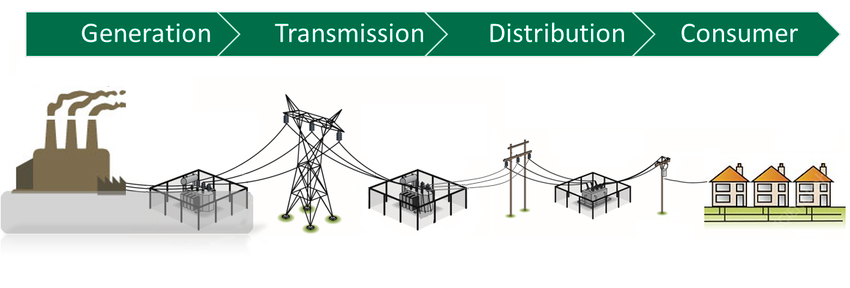
\includegraphics[width=0.98\linewidth]{imgs/grid1.jpg}
    \caption{Description of the \gls{EPS}.}
    \label{fig:grid}
\end{figure}

The growing demand for power consumption, driven by factors such as population growth, industrial advancements, and increased use of electric vehicles, combined with the rise in renewable energy sources and distributed generators spread across the electrical system, makes it necessary to implement more efficient and proactive grid management. In this context, the deployment of \gls{AMI} is a fundamental step in upgrading the \gls{EPS} to a SG, as the data collected from the consumer side can be utilized by the utility company to enhance the quality of the service provided~\cite{das2022quality}.

\gls{AMI} is an integrated network system that enables bidirectional communication between the utility company and its customers. The primary component of an \gls{AMI} system is the \gls{SMs}, which are devices installed in homes, businesses, and industries to collect data such as power consumption, voltage, and current measurements. In addition, \gls{SMs} are equipped with communication interfaces that transmit data to \gls{DAPs}, which then forward the received data to the utility company~\cite{kabalci2020smart}. Through this process, \gls{AMI} not only collects, stores, and analyzes energy usage data but also presents it in a way that enables utility companies to monitor electricity consumption, predict and detect operational failures, and identify improvements to enhance the electrical system~\cite{nashiruddin2021LoRa}.

The architecture of an \gls{AMI} is depicted in Figure~\ref{fig:ami} and consists of various \gls{SMs} distributed across the \gls{HAN}, \gls{BAN}, and \gls{IAN}, which communicate with \gls{DAPs} to transmit sensed data to concentrators, which then send the data through a \gls{WAN} connection to cloud applications managed by the utility company. The \gls{HAN} refers to the implementation of \gls{AMI} applications in homes, condominiums, and residential buildings. The \gls{BAN} involves \gls{AMI} sensor operations in commercial buildings, schools, and hospitals, while the \gls{IAN} represents the part of the \gls{AMI} system responsible for communication between the utility and industrial environments, such as factories, manufacturing plants, and other industrial facilities~\cite{veloso2021hydsmaas}.

\begin{figure}[ht]
    \centering
    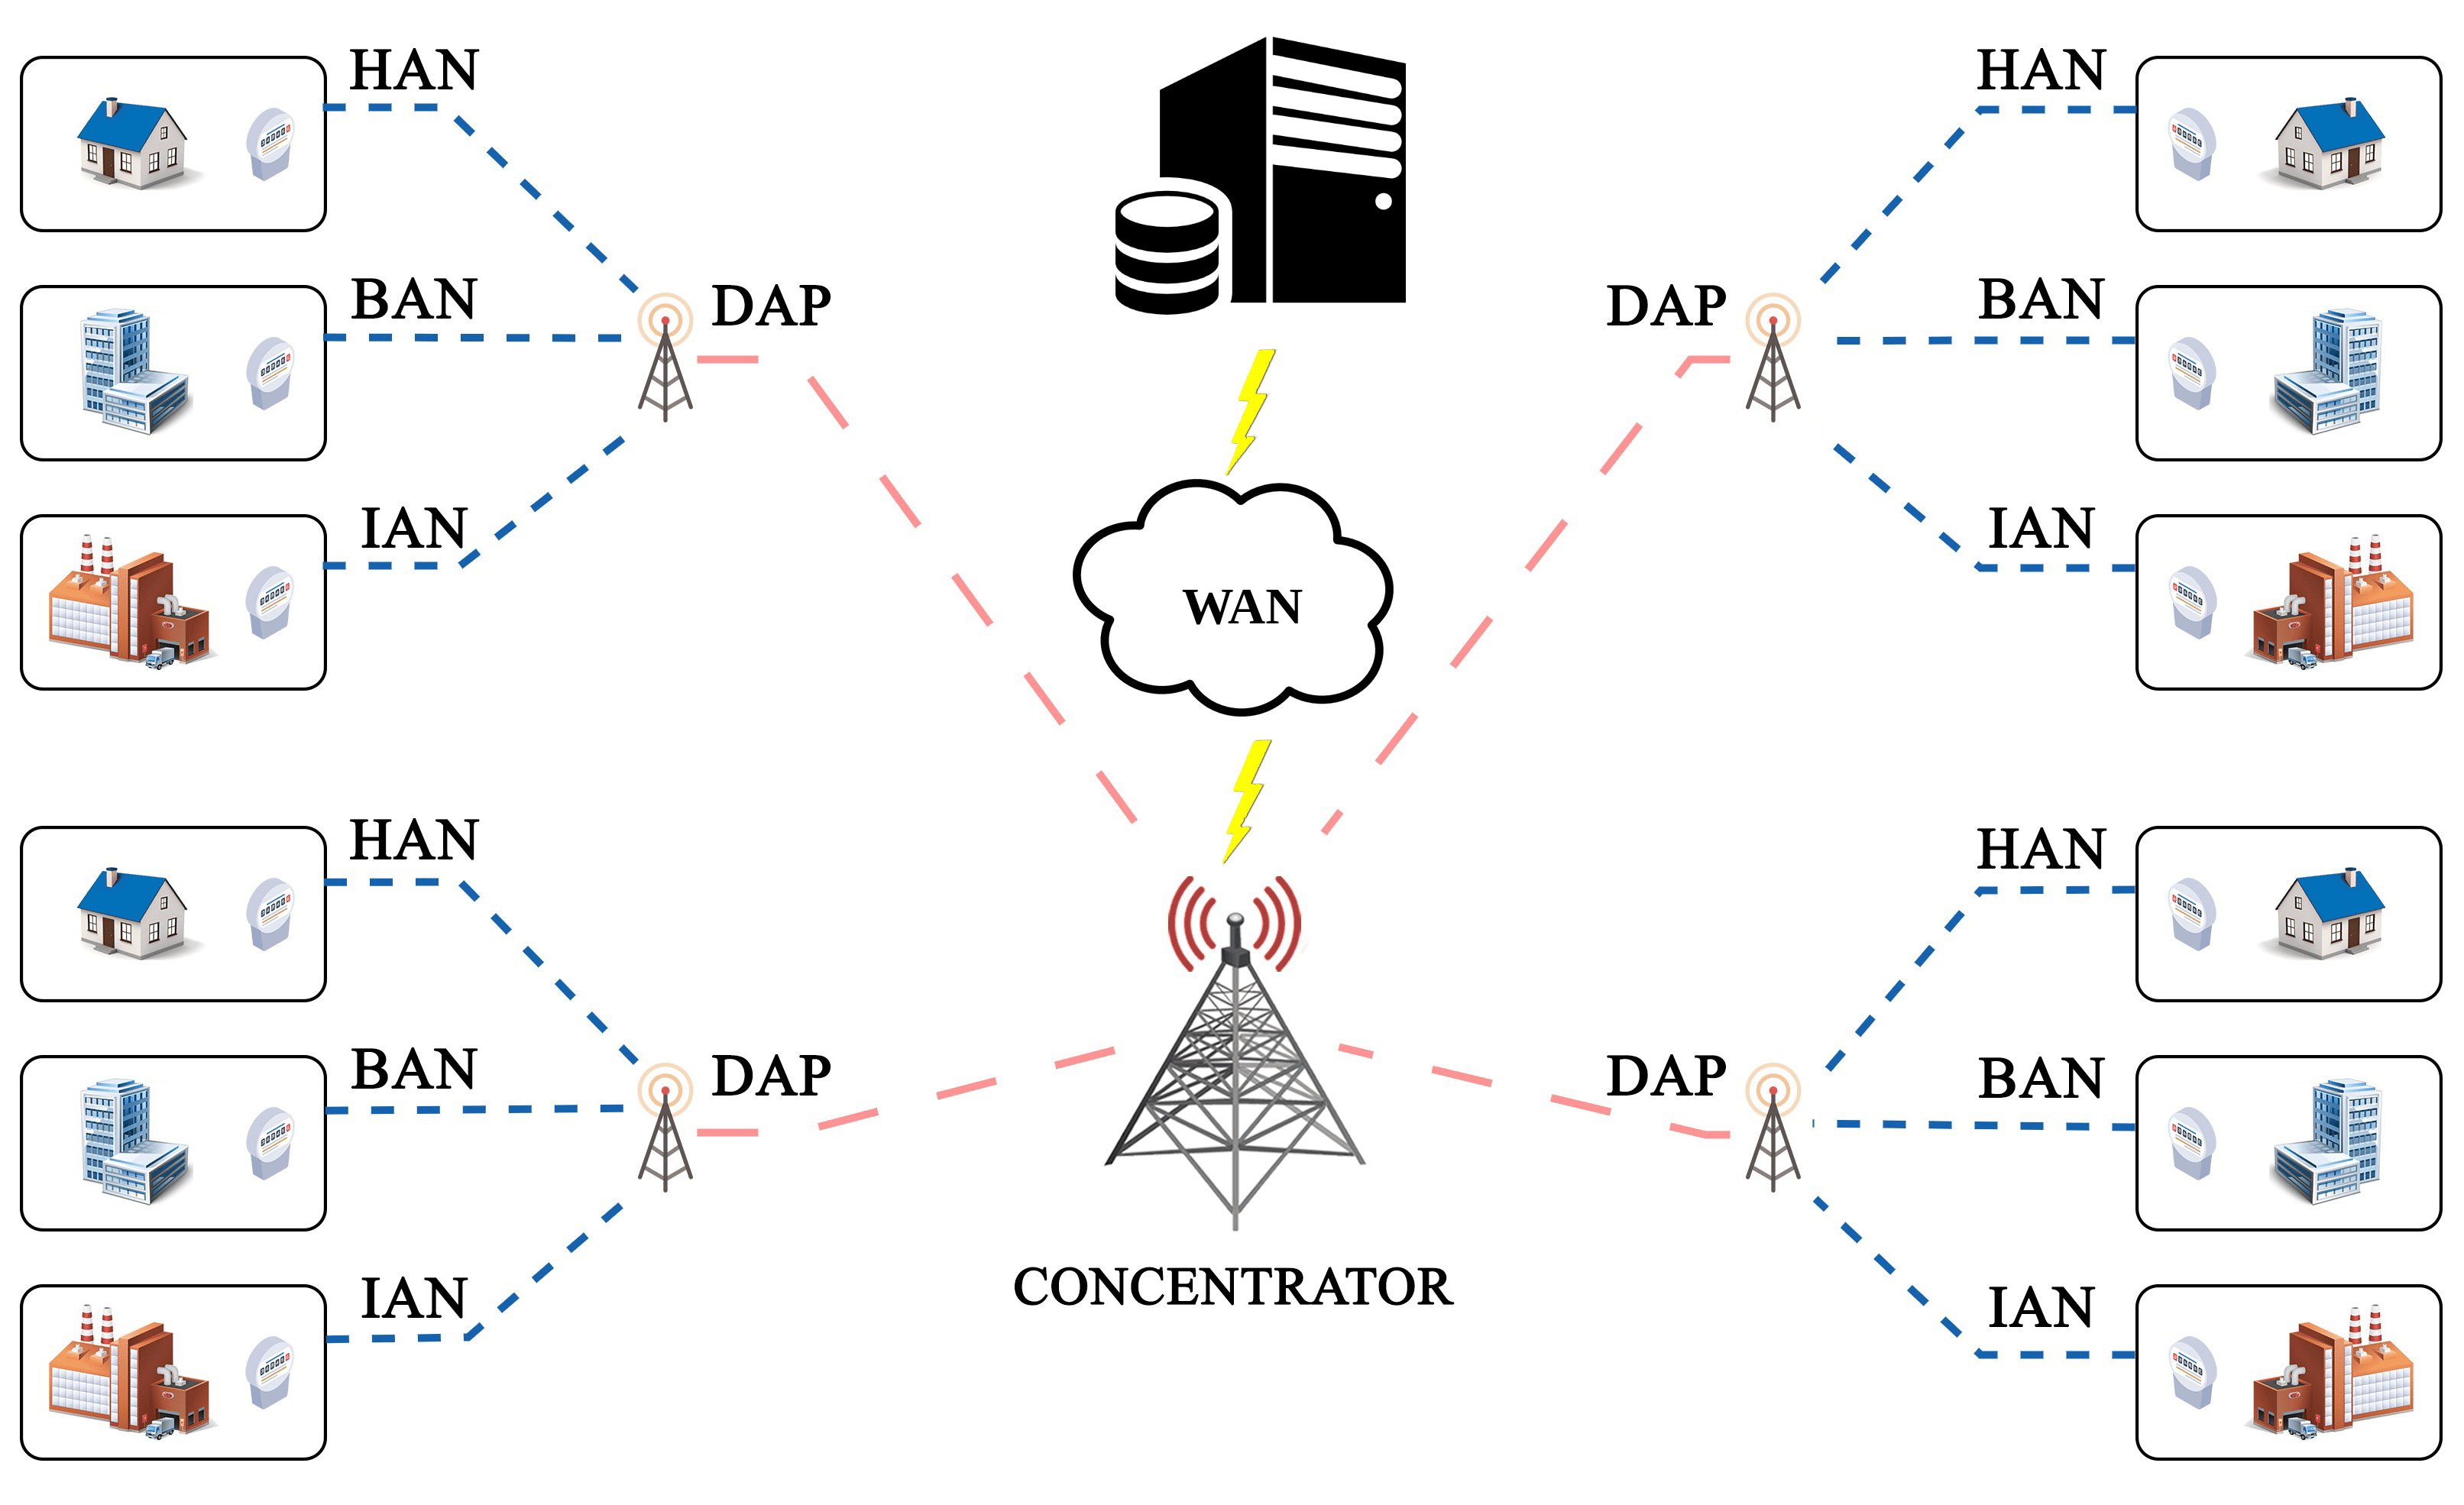
\includegraphics[width=0.98\linewidth]{imgs/ami.png}
    \caption{Architecture of the \gls{AMI} System.}
    \label{fig:ami}
\end{figure}

The operation of an \gls{AMI}, and of a SG in general, requires the use of an appropriate communication infrastructure that meets the specific needs of the applications being executed, ensuring that the services provided are beneficial to both consumers and the utility company. In this context, there is still no standardization regarding which technology should be used in each case. As a result, many proposals have been developed related to the application of wired technologies, such as Power Line Communication, and wireless standards, including mobile networks and \gls{IoT} technologies like \gls{LPWAN} networks~\cite{mohapatra2021fault}.

Moreover, in the context of AMI, various applications coexist and can be classified into normal and critical traffic classes. The normal traffic includes applications such as \gls{IMRs} and Billing Info. The IMR represents the customer electricity consumption, typically captured at fixed intervals (for example, between 5 to 60 minutes). The Billing Info involves the collection, processing, and management of data related to energy consumption, which are used to generate bills and financial reports. Similarly, the critical traffic consists of \gls{RCCs}, \gls{PCCs}, and \gls{ANs}. \gls{RCCs} include messages for disconnecting and reconnecting equipment, \gls{PCCs} receive messages to execute load control actions, and \gls{ANs} transmit messages related to meter tampering and similar issues. These applications have \gls{QoS} requirements that must be met for them to operate correctly, primarily concerning the maximum delay and the reliability rate in packet transmission, as established in~\cite{khan2022qos, khan2023qos} and displayed in Table~\ref{tab:app_qos}.

\begin{table}[ht]
    \centering
    \caption{\gls{QoS} Requirements of \gls{AMI} Applications.}
    \begin{tabular}{ccc}
        \hline \hline
        Application & Delay (seconds) & Reliability (\%) \\ \hline
        IMR & 60 & 99--99.9\\
        Billing Info & 60 & 99--99.9\\
        RCC & 1 & 99 \\ 
        PCC & 1 & 99 \\ 
        AN & 3 & 99--99.9\\ \hline \hline
    \end{tabular}
    \label{tab:app_qos}
\end{table}

\subsection{LoRaWAN} \label{sec:lorawan}

\gls{LoRaWAN} is an \gls{IoT} technology that belongs to the class of \gls{LPWAN} networks. It is characterized, especially, by its long-range coverage, low power consumption, and low deployment cost, in addition to operating in license-free \gls{ISM} bands. The \gls{LoRaWAN} protocol stack utilizes \gls{LoRa} as a physical layer technology, which provides reliable communication under harsh link conditions. The modulation scheme used in LoRa is the chirp spread spectrum (CSS), in which each \gls{LoRa} signal is divided into multiple pieces of information, each called a chirp, which consists of the transmitted symbol. For these reasons, this technology has been widely adopted in various \gls{IoT} applications, such as precision agriculture, industrial control, and smart metering~\cite{jouhari2023lorawan}.

The typical architecture of a \gls{LoRaWAN} network is based on a star topology consisting of \gls{EDs}, \gls{GWs}, the \gls{NS}, and the \gls{AS}, as described by \cite{delgado2022lorawan} and illustrated in Figure~\ref{fig:lorawan-arch}:

\begin{itemize}
    \item ED: low-power communication devices that collects data from sensors.
    \item GW: receives transmissions from the \gls{EDs} and forwards the information to the \gls{NS} and vice versa. Its functionality is similar to that of a bridge.
    \item \gls{NS}: routes the information packets between the \gls{EDs} and the \gls{AS}, depending on the predefined topic or application.
    \item \gls{AS}: responsible for ensuring that the data collected by the \gls{EDs} are correctly processed, managed, and forwarded to the end applications.
\end{itemize}

\begin{figure}[ht]
    \centering
    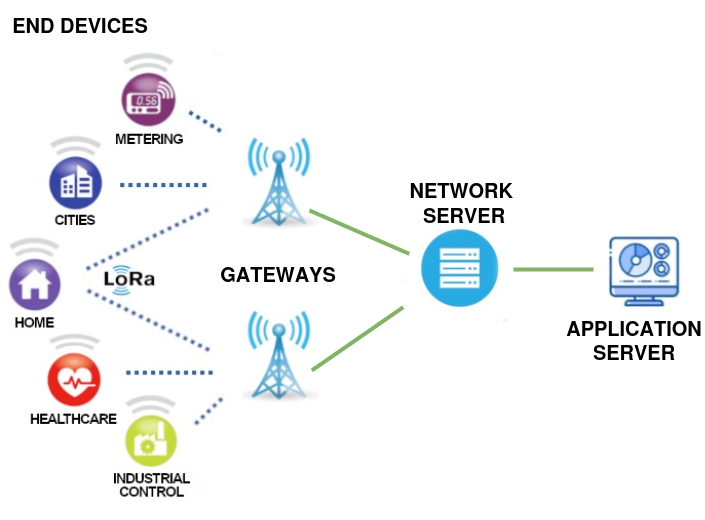
\includegraphics[width=0.98\linewidth]{imgs/lorawan.png}
    \caption{Architecture of the \gls{LoRaWAN} Network.}
    \label{fig:lorawan-arch}
\end{figure}

Some important parameters for the operation of \gls{LoRaWAN} technology include \gls{SF}, \gls{CR}, and \gls{BW}~\cite{al2024lpwan}:

\begin{itemize}
    \item The \gls{SF} is the parameter that determines how much the \gls{LoRa} signal is spread relative to its transmission time, with values ranging from 7 to 12. Generally, a higher \gls{SF} results in greater resistance to interference and better range but reduces the data transmission rate and increases energy consumption.

    \item The \gls{CR} helps improve the reliability of communication and is represented as a fraction (for example, 4/5 or 4/8), varying from 1 to 4. A higher \gls{CR} indicates more redundancy bits, resulting in greater resilience to errors but a lower data transmission rate. For instance, a \gls{CR} of 4/5 sends 4 data bits and 1 redundancy bit for error correction.

    \item \gls{BW} refers to the amount of frequency spectrum used for transmission. Common options include 125 kHz, 250 kHz, and 500 kHz. \gls{BW} influences the data rate and signal sensitivity.
\end{itemize}

In \gls{LoRaWAN}, each symbol represents a number of transmitted bits, denoted as \(N_{bits}\), as expressed by Equation~\ref{eq:nbits}. Thus, each symbol for SF7 transmits 7 bits, while SF12 transmits 12 bits~\cite{montagny2021lora, marini2022lpwan}.

\begin{equation} \label{eq:nbits}
    N_{bits} = \text{SF}
\end{equation}

The \gls{DR} in a LoRaWAN network is determined by several parameters, including the \gls{SF}, \gls{CR}, and \gls{BW}. The general formula for calculating the \gls{DR} in a \gls{LoRaWAN} network is expressed in Equation~\ref{eq:dr}:

\begin{equation} \label{eq:dr}
    \text{DR} = \text{SF} \cdot \frac{\text{\gls{BW}}}{2^{\text{SF}}} \cdot \text{CR}
\end{equation}

The transmission time of each symbol, \( T_{symbol} \), depends on the \gls{SF}. The higher the \gls{SF}, the longer the transmission time, as presented in Equation~\ref{eq:t-symbol}. For the same \gls{BW}, for example, the transmission time of a symbol in SF8 is twice as long as that of a symbol in SF7~\cite{montagny2021lora, marini2022lpwan}.

\begin{equation} \label{eq:t-symbol}
    T_{symbol} = \frac {2^{\text{SF}}} {\text{\gls{BW}}}
\end{equation}

Another important factor in the \gls{LoRaWAN} network \gls{ToA}, which consists of the overall duration of a \gls{LoRaWAN} frame; that is, the time it takes for a frame to be transmitted over the air, from the beginning of transmission to the end, and it is calculated as per Equation~\ref{eq:toa}.

\begin{equation} \label{eq:toa}
    \text{ToA} = T_{premble} + T_{payload}
\end{equation}

\noindent where \( T_{\text{preamble}} \) is the duration of the preamble symbol and \( T_{\text{payload}} \) is the duration of the payload of the frame.

The \gls{ToA} of the preamble depends on the number of symbols in the preamble, \( n_{\text{preamble}} \), and is obtained using Equation~\ref{eq:toa-preamble}. For the EU-868 region, which includes Europe, \( n_{\text{preamble}} = 8 \).

\begin{equation} \label{eq:toa-preamble}
    T_{\text{preamble}} = \left( n_{\text{preamble}} + 4.25 \right) \cdot T_{\text{symbol}}
\end{equation}

In turn, the duration of the payload, \( T_{\text{payload}} \), is calculated using Equation~\ref{toa-payload}.

\begin{equation} \label{toa-payload}
    T_{\text{payload}} = n_{\text{payload}} \cdot T_{\text{symbol}}
\end{equation}

\noindent where \( n_{\text{payload}} \) is the number of symbols in the payload of the physical layer data unit, calculated using Equation~\ref{n-payload} and depending on the packet size, headers, and the CRC field.

% \begin{equation} \label{n-payload}
%     n_{\text{payload}} = \max \left[ \lceil \frac{8 \cdot \text{PL} - 4 \cdot \text{SF} + 28 + 16 - 20 \cdot \text{H}}{4 \cdot (\text{SF} - 2 \cdot \text{DE})} \rceil \cdot (\text{CR} + 4), 0 \right]
% \end{equation}
\begin{equation} \label{n-payload}
    n_{\text{payload}} = \max \left[ 
    \begin{split}
        \lceil \frac{8 \cdot \text{PL} - 4 \cdot \text{SF} + 28 + 16 - 20 \cdot \text{H}}{4 \cdot (\text{SF} - 2 \cdot \text{DE})} \rceil \\
        \cdot~(\text{CR} + 4), 0 
    \end{split}
    \right]
\end{equation}



\noindent where \(\text{PL}\) is the packet size, \(\text{H} = 0\) when the header is enabled and \(\text{H} = 1\) when no header is present, \(\text{DE} = 1\) when low data rate optimization is enabled and \(\text{DE} = 0\) when it is disabled, and \(\text{CR}\) is the coding rate from 1 to 4.

LoRaWAN defines three classes of \gls{EDs} that meet different operational and energy efficiency requirements~\cite{elbsir2023evaluation}:

\begin{itemize}
    \item Class A (All): The default class, in which the ED opens two reception windows -- RX1 and RX2 -- after transmitting an uplink message. These reception windows are used to receive downlink messages, such as messages sent by the \gls{NS} for the ED to adjust its \gls{SF} to a new value. This class consumes the least energy, making it ideal for low-power devices, such as battery-powered sensors in remote locations that send data sporadically.

    \item Class B (Beacon): This class allows \gls{EDs} to open additional reception windows at regular intervals, synchronized based on prior uplink communication. The \gls{GWs} periodically send beacons, as determined by the \gls{NS}, instructing the ED to open additional reception windows. This class provides a greater opportunity to receive downlink data, but increases energy consumption. It is suitable for sensors that collect data but also need to be available for specific actions at certain times.

    \item Class C (Continuous): This class enables the ED to continuously receive downlink data, with RX2 open until a new uplink transmission is needed. This class consumes the most energy but significantly reduces downlink latency, making it suitable for devices that require real-time communication.
\end{itemize}

Furthermore, \gls{LoRaWAN} utilizes an ALOHA-based protocol~\cite{heusse2023lorawan}, allowing \gls{EDs} to operate without the need to establish a direct connection with specific gateways, and the duty cycle is generally 1\%. Instead, all messages sent by \gls{EDs} are received by all gateways within range, which then forward these messages to the \gls{NS}. If the Network Server receives multiple copies of the same message, it stores a single copy and discards the duplicates. The communication initiated by the \gls{EDs} is referred to as uplink, while communication initiated by the \gls{NS} is known as downlink. Downlink messages may transmit \gls{ACK} for received uplink messages or adjustments to the operational parameters of the \gls{EDs}~\cite{marini2022lpwan}.


% Adicionalmente, o tráfego de dados na rede LoRAWAN pode funcionar no modo padrão \gls{NACK}, com os \gls{EDs} transmitindo dados uplink sem a necessidade de saber se estes foram recebidos corretamente, pois as aplicações executadas não possuem restrições de confiabilidade de entrega. Caso contrário, a rede \gls{LoRaWAN} pode transmitir os dados em modo \gls{ACK}. Dessa forma, como o data traffic in most \gls{IoT} applications can be grouped geralmente into three main categories: monitoring, control and safety, é necessário decicir corretamente o uso do modelo de comunicação. Monitoring includes almost unidirectional traffic originated from medições periodicas de sensores. The control category implies a feedback action on the environment, usually generated within well-defined deadlines, such as requisitos de real-time behavior. Finally, the safety category represents emergency actions after occurrence of sporadic alarm events, which require immediate reaction and \gls{ACK}~\cite{carvalho2021lorawan}. 
Additionally, data traffic in a \gls{LoRaWAN} network can be transmitted in the default \gls{NACK} mode or in \gls{ACK} mode. \gls{EDs} transmitting uplink data without confirmation are not notified if the packet was received, resulting in less network overhead. In contrast, \gls{ACK} transmissions increase the traffic load on the network in exchange for improved reliability of packet delivery. The establishment of the traffic model to be used by \gls{IoT} applications is important, as they have diverse \gls{QoS} requirements and can be grouped into three main categories: monitoring, control, and safety. Monitoring primarily includes unidirectional traffic originating from periodic sensor measurements. The control category implies feedback actions on the environment, typically within well-defined deadlines, such as requirements for real-time behavior. Finally, the safety category represents emergency actions triggered by sporadic alarm events, which require immediate reaction and \gls{ACK}~\cite{carvalho2021lorawan}.

% O uso de comunicação \gls{ACK} permite que um mesmo pacote possa ser transmitido até 8 vezes: 1 transmissão inicial, mais 7 possíveis retransmissões. Ou seja, o ED transmiste uma mensagem e espera a chegada do \gls{ACK} em uma mensagem downlink e, caso essa mensagem não seja recebida até o final da duração de RX1 ou de RX2, o ED pode retransmitir o pacote. Se a mensagem de \gls{ACK} for recebida logo após a primeira transmissão, ou antes da sétima retransmissão, o pacote confirmado não é mais enviado. Assim, a rede \gls{LoRaWAN} incrementa a garantia de confibilidadede entrega de pacotes e também prejudica a transmissão \gls{NACK}, pois a operação padrão do \gls{LoRaWAN} especifica que o tráfego \gls{ACK} deve ser priorizado em detrimento do \gls{NACK}. Assim, nos cenários que executam aplicações \gls{IoT} com mixed-criticality, tais como sistema de health, industriais e de medição inteligente, as three categories descritas anteriormente devem coexistir e, consequentemente tráfego \gls{ACK} e \gls{NACK} devem ser utilizados simultaneamente~\cite{wei2023priority}.
The use of \gls{ACK} communication allows the same packet to be transmitted up to 8 times: 1 initial transmission, plus 7 possible retransmissions. In this case, the ED sends a message and waits for the \gls{ACK} in a downlink message. If this message is not received by the ED in one of the reception windows, the packet is retransmitted. If the \gls{ACK} message is received right after the first transmission, or before the seventh retransmission, the confirmed packet is no longer sent. Thus, the \gls{LoRaWAN} network increases the reliability of packet delivery but also impacts \gls{NACK} transmission. This is caused by the standard operating mode of \gls{LoRaWAN}, which specifies that \gls{ACK} traffic must be prioritized over \gls{NACK}. In systems running \gls{IoT} applications with mixed criticality, such as health, industrial, and smart metering, the three categories described earlier must coexist, and consequently, both \gls{ACK} and \gls{NACK} traffic must be used simultaneously~\cite{wei2023priority}.

% \begin{itemize}
%     \item Classe A (All): classe padrão e funciona com o ED abrindo duas janelas de recepção -- RX1 e RX2 -- após transmitir uma mensagem de uplink. Essa janelas de recepção são utilizadas para receber mensagens downlink, tais como mensagem \gls{ACK} enviadas pelo \gls{NS}, notificando que a mensagem uplink foi recebida corretamente. Essa classe é a que menos gasta energia, sendo ideal para dispositivos com baixo consumo de energia, alimentados por bateria por exemplo, como sensores em locais remotos que enviam dados esporadicamente.

%     \item Classe B (Beacon): classe que proporciona aos \gls{EDs} abrirem além das duas janelas de recepção padrão, janelas adicionais em intervalos regulares sincronizadas a partir de comunicação uplink prévia. Então, os \gls{GWs} enviam beacons de sinalização periodicamente, de acordo com determinação dos \gls{NS}, indicando ao ED abrir janelas adicionais de recepção. Essa classe proporciona uma maior possibilidade de  receber dados downlink e, em contrapartida aumenta o consumo energético, sendo indicada para sensores que coletam dados, mas que também precisam estar disponíveis para serem acionados em momentos específicos.

%     \item Classe C (Continuous): classe que proporciona ao ED a possibilidade de recepção contínua de dados downlink, com RX2 aberta continuamente até um nova transmissão uplink ser necessária, execeto quando a janela RX1 é aberta. Esse classe consomem mais energia, reduz drasticamente a latência na recepção de dados downlink, consumindo o maior nível de energia em comparação as outras classes e é adequada para dispositivos que precisam de comunicação em tempo real.
% \end{itemize}

\section{Clustering} \label{sec:clustering}

Clustering is an unsupervised learning technique used to identify patterns and discover knowledge by classifying unlabeled data based on their similarities. This technique has been successfully applied to address data clustering problems across various domains, including medical science, manufacturing, power grids, robotics, the financial sector, privacy protection, urban development, aviation, as well as in industries such as sales and marketing, among many others~\cite{mandhi2021clustering}. For this reason, many studies have applied this technique in the planning of \gls{LoRaWAN} networks~\cite{matni2020lorawan, neriPerformance2022} and communication infrastructures for \gls{SGs}~\cite{si2021clustering, alonso2022clustering, piechowiak2023lorawan, gallardo2021clustering}.

Moreover, clustering algorithms can be classified in several ways, often based on the method of cluster formation. One of the most common classifications in the literature distinguishes between hard and soft clustering. In the hard approach, each object is assigned to one and only one cluster. Conversely, in the soft approach, an object can belong to multiple clusters with varying degrees of membership. A data point can be allocated to a particular cluster if the membership value associated with that group is the highest among all obtained from the clustering method. For instance, in fuzzy clustering, each data point is assigned a degree of membership that quantifies its belonging to each cluster~\cite{oyewole2023data}.

There are numerous hard and soft clustering algorithms available. To simplify the presentation of examples from both types, this paper introduces the algorithms employed in the clustering process of the proposed method, as well as those from related works discussed in Section~\ref{sec:works}. Initially, the hard clustering algorithms K-Means and K-Medoids will be presented, followed by the soft clustering algorithm Fuzzy C-Means.

\subsection{K-Means}

K-Means is an iterative algorithm used to form clusters from a dataset. This algorithm stores $k$ centroids that it uses to define clusters. A point is considered to be in a particular cluster if it is closer to that cluster centroid than any other centroid. Thus, it can be described by the following steps according to~\cite{yang2023unsupervised}:

\begin{itemize}
    \item Step 1: Select \( k \) random points from the dataset as the initial centroids of the clusters.
    
    \item Step 2: For each data point in the dataset, compute the distance between the point and each centroid. Assign each point to the cluster whose centroid is closest, typically using a distance metric such as the Euclidean distance.
    
    \item Step 3: Recalculate the position of the centroids for each cluster. The new centroid is the mean (or center) of all points assigned to that cluster.
    
    \item Step 4: Repeat steps 2 and 3 until the centroids do not change significantly, or until a maximum number of iterations is reached. This indicates that the clusters have stabilized.
\end{itemize}

\subsection{K-Medoids}

The K-Medoids algorithm is a clustering technique similar to K-Means, where the central points of the clusters are referred to as medoids. Each point is an actual object from the dataset rather than an average of the objects within the cluster. The medoid of a cluster is defined as the object in the cluster with the minimum average dissimilarity to all other objects in that cluster, meaning it is the most centrally located point within the cluster. An overview description of this algorithm is presented below, according to~\cite{gallardo2021clustering}:

\begin{itemize}
    \item Step 1: Select \( k \) random points from the dataset as the initial medoids.

    \item Step 2: For each point in the dataset, calculate the distance between that point and each of the medoids. Assign each point to the cluster whose medoid is closest, using a distance measure, which is typically the Euclidean distance.

    \item Step 3: For each cluster, find the point that minimizes the sum of distances between it and all other points in the cluster. This point becomes the new medoid of the cluster.

    \item Step 4: Repeat Steps 2 and 3 until the medoids do not change significantly or until a maximum number of iterations is reached. This indicates that the clusters have stabilized.
\end{itemize}

\subsection{Fuzzy C-Means}

The Fuzzy C-Means algorithm is an unsupervised clustering method that enables the creation of a fuzzy partition from data. The algorithm relies on a parameter \( m \), which represents the fuzziness weighting exponent used to update the degree of membership. Fuzzy C-Means has been extensively applied in clustering, classification, and pattern recognition. The steps of the algorithm are outlined below, as described in~\cite{oyewole2023data}:

\begin{itemize}
    \item Step 1: Initialize the \(U\) partition matrix with random numbers in the range \([0, 1]\), representing the degrees of membership of each data point with respect to all the clusters to be generated.
    
    \item Step 2: Calculate the centroids of the clusters, using Equation~\ref{eq:fcm_centers}.

    \begin{equation} \label{eq:fcm_centers}
        v_j = \frac{\sum_{i=1}^{n} u_{ij}^m \cdot x_i}{\sum_{i=1}^{n} u_{ij}^m}
    \end{equation}

    where \(v_j\) is the center of cluster \(j\), \(u_{ij}\) is the membership degree of data point \(x_i\) to cluster \(j\), \(x_i\) is the data point, and \(n\) is the number of data points.

    \item Step 3: Recalculate the degrees of membership \(u_{ij}\) based on the new distances of the points to the cluster centers, using Equation~\ref{eq:fcm_member}. 

    \begin{equation} \label{eq:fcm_member}
        u_{ij} = \left( \sum_{k=1}^{c} \left( \frac{\lVert x_i - v_j \rVert}{\lVert x_i - v_k \rVert} \right)^{\frac{2}{m-1}} \right)^{-1}
    \end{equation}

    where \(u_{ij}\) is the membership degree of data point \(x_i\) to cluster \(j\), \(v_j\) is the center of cluster \(j\), \(x_i\) is the data point, and \(c\) is the number of clusters.
    
    \item Step 4: Calculate the objective function using Equation~\ref{eq:fcm_obj}.

    \begin{equation} \label{eq:fcm_obj}
        J(U, V) = \sum_{i=1}^{n} \sum_{j=1}^{c} u_{ij}^m \cdot \lVert x_i - v_j \rVert^2
    \end{equation}

    where \(J(U, V)\) is the objective function to be minimized, \(u_{ij}^m\) is the membership degree of data point \(x_i\) to cluster \(j\) raised to the power of \(m\), \(\lVert x_i - v_j \rVert^2\) is the squared distance between data point \(x_i\) and cluster center \(v_j\), \(n\) is the number of data points, and \(c\) is the number of clusters.

    \item Step 5: The algorithm stops when the difference between the membership matrices from two consecutive iterations becomes smaller than the tolerance value \(\epsilon\), as described in Equation~\ref{eq:convergence}. Otherwise, it returns to Step 2.

    \begin{equation} \label{eq:convergence}
        \lVert U^{(t+1)} - U^{(t)} \rVert < \epsilon
    \end{equation}

    where \(\lVert U^{(t+1)} - U^{(t)} \rVert\) is the norm representing the difference between the membership matrices at iteration \(t+1\) and iteration \(t\), \(\epsilon\) is the predefined tolerance threshold (a small positive value), and \(U^{(t)}\) and \(U^{(t+1)}\) are the membership matrices at iteration \(t\) and \(t+1\), respectively.
\end{itemize}

\section{Method Description} \label{sec:method}

The proposed method operates iteratively, and each iteration defines a set \(k\) of clusters of \gls{SMs}, with the coordinates of the centroids corresponding to the positions of the \gls{DAPs}, as shown in Figure~\ref{fig:scenario}. The method takes as inputs the initial value of \(k\), the coordinates of the SMs, \text{smCoords}, as well as the minimum PDR value, \text{minPdr}, and maximum delay, \text{maxDelay}, which establish the \gls{QoS} constraints for the \gls{AMI} applications.

\begin{figure}[ht]
    \centering
    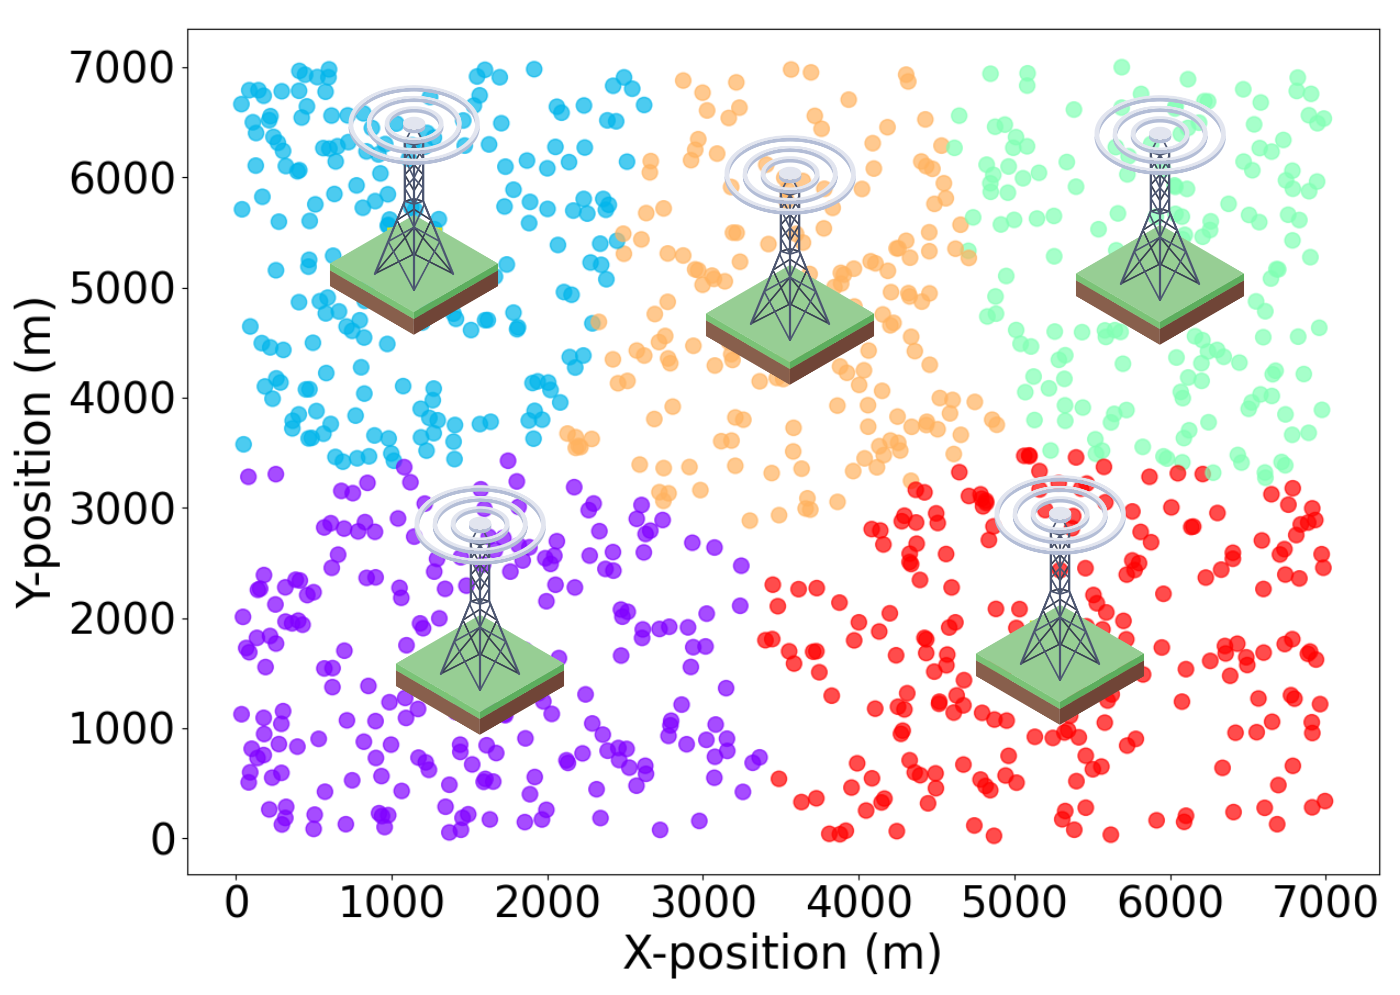
\includegraphics[width=0.98\linewidth]{imgs/5gws.png}
    \caption{Example of AMI Scenario.}
    \label{fig:scenario}
\end{figure}

% O funcionamento do método proposto, denominado cPlace, segue o fluxograma descrito na Figura~5. Inicialmente, na etapa de Geração das Coordenadas dos \gls{SMs}, as coordenadas x e y dos \gls{SMs} são geradas aleatoriamente via código em Python~\cite{python2022} dentro dos limites da área de teste a ser simulada e estas juntamente com o valor de \( k \) são passadas a próxima etapa. Então, o método segue a etapa de Clusterização e o algoritmo Fuzzy C-Means é executado com a utilização da biblioteca skfuzzy\footnote{https://pythonhosted.org/scikit-fuzzy/}, para definir uma quantidade \( k \) inicial de clusters, denotada como labels, de \gls{SMs} com os \gls{DAPs} como centróides, utilizando o exponente de fuzzificação com valor igual a 2. Além disso, o método considera que um SM é alocado ao cluster com o qual ele possui maior grau de pertinência e as coordenadas dos \gls{DAPs}, dapCoords, são estabelecidas com base nas coordenadas dos \gls{SMs}.
The operation of the proposed method, called cPlace, follows the flowchart described in Figure~\ref{fig:flowchart}. Initially, in the Coordinate Generation of the \gls{SMs} step, the x and y coordinates of the \gls{SMs} are randomly generated using Python code~\cite{python2022} within the boundaries of the test area to be simulated, and these, along with the value of \( k \), are passed to the next step. Then, the method proceeds to the Clustering step, where the Fuzzy C-Means algorithm is executed using the skfuzzy library\footnote{https://pythonhosted.org/scikit-fuzzy/}, to define an initial quantity \( k \) of clusters, denoted as labels, of SMs with the \gls{DAPs} as centroids, using a fuzzification exponent, $m$, set to 2. Additionally, the method considers that an SM is allocated to the cluster with which it has the highest degree of membership, and the coordinates of the \gls{DAPs}, dapCoords, are established based on the coordinates of the \gls{SMs}.

\begin{figure}[ht]
    \centering
    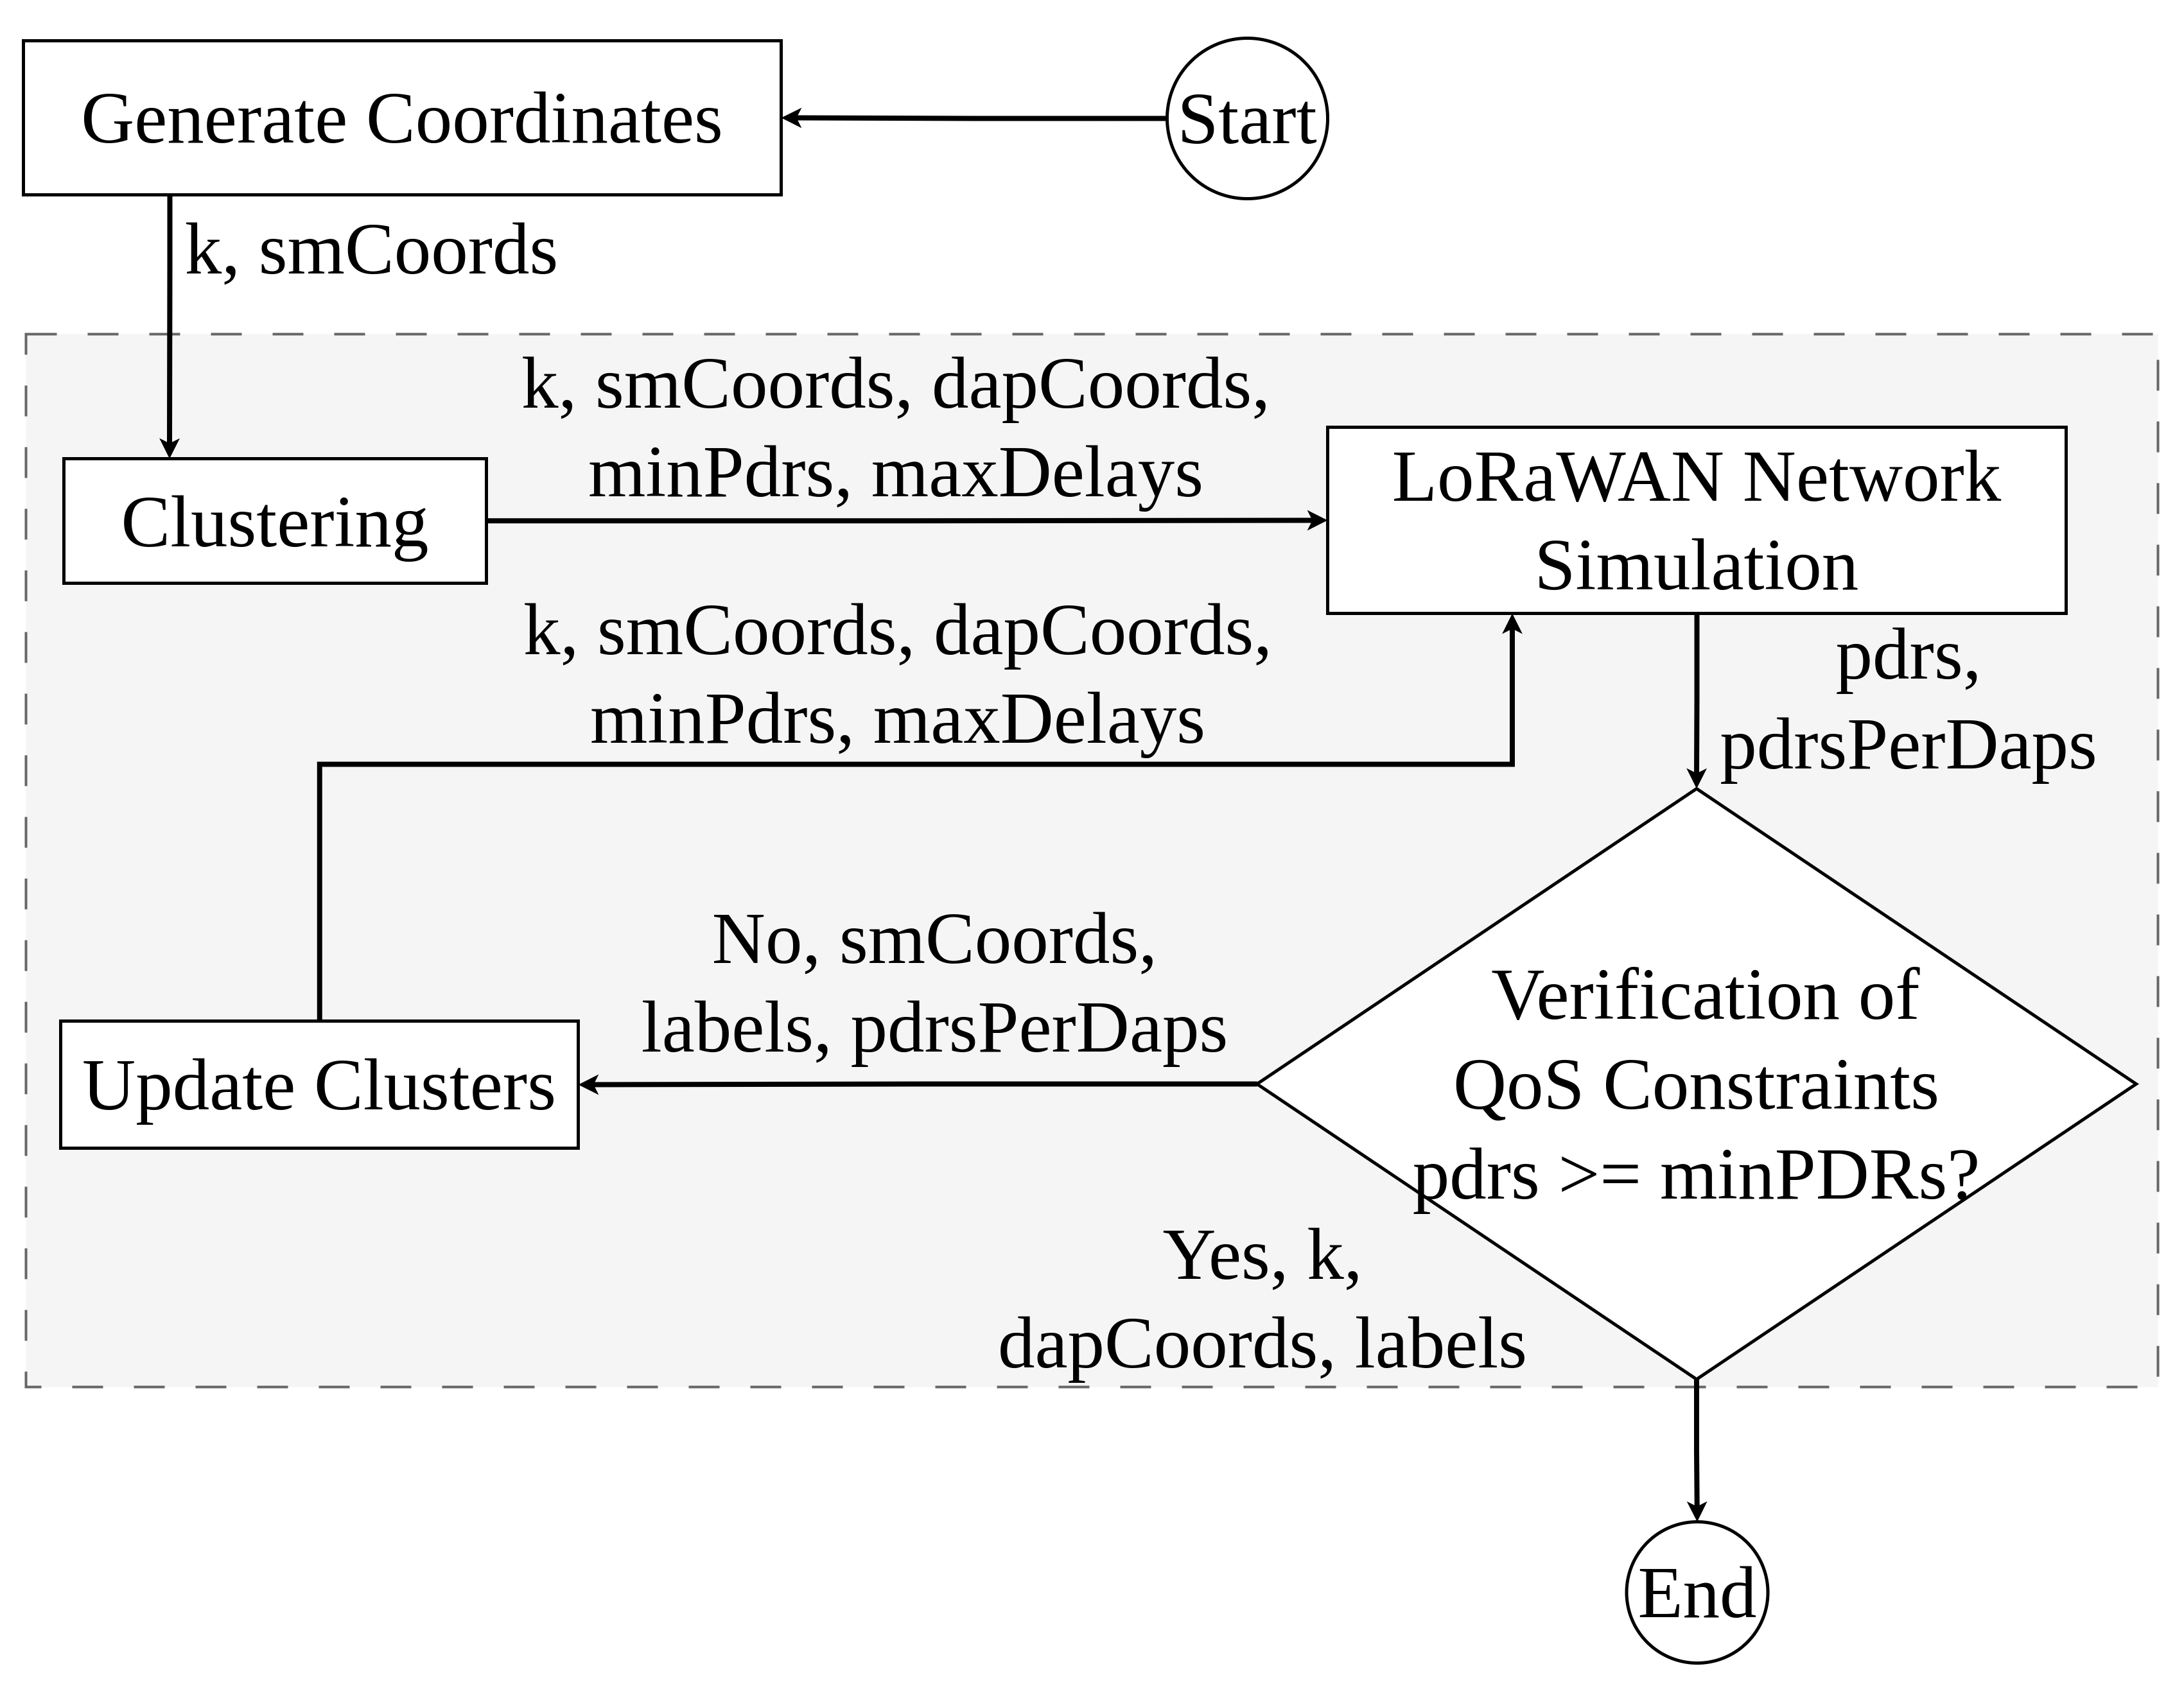
\includegraphics[width=1\linewidth]{imgs/flowchart.png}
    \caption{Flowchart Depicting the Sequence of Steps of the cPlace Method.}
    \label{fig:flowchart}
\end{figure}

% Em seguida, o método segue para a etapa de Simulação da Rede LoRaWAN, que recebe como entradas \( k \), smCoords, dapCoords, e labels. Os \gls{SMs} e \gls{DAPs} são posicionados no cenário, as aplicações \gls{AMI} são instaladas nos \gls{SMs} considerando as requisitos de \gls{QoS} citadas na Seção~\ref{sec:ami}, os \gls{SMs} e \gls{DAPs} são conectados através de \gls{LoRaWAN}, e a simulação é executada gerando como saída os valores das métricas de avaliação descritas na Seção~\ref{sec:metrics}.
Next, the method proceeds to the \gls{LoRaWAN} Network Simulation step, which takes as inputs \( k \), smCoords, dapCoords, and labels. The \gls{SMs} and DAP are positioned in the scenario, the \gls{AMI} applications are installed on the \gls{SMs}, considering the \gls{QoS} requirements mentioned in Section~\ref{sec:ami}, the \gls{SMs} and \gls{DAPs} are connected via \gls{LoRaWAN}, and the simulation is run, generating as output the evaluation metric values described in Section~\ref{sec:metrics}.

% Posteriormente, o método chega a etapa de Verificação das Restrições de \gls{QoS}, que determina se a taxa de confiabilidade mínima e o delay máximo das aplicações foram satistfeitas. Se nenhuma restrição tiver sido violada, o método chega ao fim de sua execução e retorna para o planejamento da infraestrutura de comunicação \gls{IoT} \( k \), labels, e dapCoords. Caso contrário, a método passa a etapa de Atualização dos Clusters, com base na  utilização da métrica \gls{PDR}, que consiste na taxa de pacotes recebidos com sucesso pelos \gls{DAPs} dentro do limite máximo de delay exigido pelas aplicações, e usa o \gls{PDR} para atualizar os \gls{SMs} que formam cada cluster e as coordenadas x e y dos \gls{DAPs}.
Subsequently, the method reaches the Verification of \gls{QoS} Constraints step, which determines whether the minimum reliability rate and the maximum delay of the applications have been satisfied. If no constraint has been violated, the method concludes its execution and returns the IoT communication infrastructure plan with \( k \), labels, and dapCoords. Otherwise, the method moves to the Cluster Update step, based on the \gls{PDR} metric, which represents the rate of packets successfully received by the \gls{DAPs} within the maximum delay required by the applications. The \gls{PDR} is used to update the \gls{SMs} that form each cluster and the x and y coordinates of the \gls{DAPs}.

% O \gls{PDR} é aplicado da seguinte forma: um SM é alocado ao cluster cujo DAP recebeu com sucesso a maior quantidade de mensagens enviadas pelo SM e em tempo hábil. Assim, se o DAP$_{5}$ obteve o maior valor de \gls{PDR} para as mensagens enviadas pelo SM$_{1}$, o SM$_{1}$ é adicionado ao cluster 5 e as coordenadas do DAP$_{5}$ são atualizadas como a média das coordenadas de todos os \gls{SMs} que agora fazem parte do cluster $5$. Com isso, pretende-se mover os \gls{DAPs} para posições que podem alcançar uma maior taxa de recepeção bem-sucedida de pacotes. Após os clusters e as coordenadas dos \gls{DAPs} serem atualizadas a método volta a etapa de Simulação da Rede LoRaWAN.
The \gls{PDR} is applied as follows: an SM is allocated to the cluster whose DAP successfully received the highest number of messages sent by the SM in a timely manner. Thus, if DAP$_{5}$ achieved the highest \gls{PDR} value for the messages sent by SM$_{1}$, SM$_{1}$ is added to cluster 5, and the coordinates of DAP$_{5}$ are updated as the average of the coordinates of all SM that now belong to cluster $5$. This approach aims to move the DAP to positions that can achieve a higher rate of successful packet reception. Once the clusters and the coordinates of the DAP are updated, the method returns to the \gls{LoRaWAN} Network Simulation step.

%A nova execução da etapa de Simulação da Rede LoRaWAN serve para verificar se os ajustes realizados na etapa de Atualização dos Clusters melhoraram os resultados de performance da comunicação. Assim, o método passa a etapa de Verificação das Restrições e caso todas as restrições de funcionamento das aplicações sejam satisfeitas o método retorna os valores \( k \), labels, e dapCoords. Caso contrário o valor de \( k \) é incrementado em uma unidade e o método volta a etapa de Clusterização.
The new execution of the \gls{LoRaWAN} Network Simulation step serves to verify whether the adjustments made during the Cluster Update step have improved the communication performance results. Thus, the method proceeds to the Verification of Constraints step, and if all application operation constraints are satisfied, the method returns the values of \( k \), labels, and dapCoords. Otherwise, the value of \( k \) is incremented by one, and the method returns to the Clustering step.

%A fim de aprimorar o entendimento do método proposto, o Algoritmo~\ref{alg:method} é apresentado, descrevendo cPlace no formato de pseudocódigo. O método recebe como entradas os valores $k$, smCoords, os valores mínimos de \gls{PDR} para cada aplicação \gls{AMI} a ser executada, denotado como minPdrs, e os valores de máximo delay requerido para cada aplicação, maxDelay.
In order to enhance the understanding of the proposed method, Algorithm~\ref{alg:method} is presented to describe cPlace in pseudocode format. The method takes as inputs the values of \( k \), smCoords, the minimum \gls{PDR} values for each \gls{AMI} application to be executed, denoted as minPdrs, and the maximum delay requirements for each application, maxDelay.

\begin{algorithm}[ht]
    \caption {kPlace Method.}
    \label{alg:method}
    
    \textbf{Inputs:} {\texttt{$k$, smCoords, minPdrs, maxDelays}}
    
    % \KwResult{Output result}
    % Initialize parameters
    
    \While {\texttt{true}} {
        \texttt{dapCoords, labels} \texttt{=} \texttt{CMeans($k$, smCoords, m=2)}
        
        \texttt{pdrs, pdrsPerDap = Simulate($k$, smCoords, dapCoords, minPdrs, maxDelays)} 

        \texttt{ok = true}
        
        \For {\texttt{i = 0; i < len(minPdrs); i++}} {
            \texttt{pdr = pdrs[i]}
            
            \If {\texttt{pdr < minPdrs[i]}} {
                \texttt{ok = false}

                \textbf{break}
            }
        }

        \If {\texttt{ok == true}} {
            \textbf{break}
        }

        \texttt{dapCoords, labels = UpdateClusters($k$, smCoords, dapCoords, pdrsPerDaps)}

        \texttt{pdrs, pdrsPerDaps = Simulate($k$, smCoords, dapCoords, minPdrs, maxDelays)}

        \texttt{ok = true}
        
        \For {\texttt{i = 0; i < len(minPdrs); i++}} {
            \texttt{pdr = PDRs[i]}
            
            \If {\texttt{pdr < minPdrs[i]}} {
                \texttt{ok = false}

                \textbf{break}
            }
        }

        \If {\texttt{ok == true}} {
            \textbf{break}
        }

        \texttt{k = k + 1}
    }
    
    \Return \texttt{$k$, dapCoords, labels}
\end{algorithm}


% A clusterização inicial utilizando o Fuzzy C-Means é executada na linha 3 e o algoritmo de clusterização recebe $k$, smCoords e $m$ igual a 2. Em seguida, na linha 4, a simulação é executada e as métricas de avaliação são geradas, sendo retornado para o método um vetor com os PDRs para cada uma das aplicações \gls{AMI} testadas. Nas linhas 6 a 10, o valor de \gls{PDR} de cada uma das aplicações, representado como pdr, é verificado se é menor ao valor mínimo exigido, e se alguma aplicação não tiver a restrição satisfeita a flag ok é setada para false. Consequentemente, o método deve atualizar os clusters através da função UpdateCluster.
The initial clustering using Fuzzy C-Means is executed on line 3, where the clustering algorithm receives \texttt{\( k \)}, \texttt{smCoords}, and \texttt{\( m \)} set to 2. Then, on line 4, the simulation is executed, generating the evaluation metrics and returning a vector of PDRs for each of the tested \gls{AMI} applications. In lines 6 to 10, the \gls{PDR} value for each application, represented as pdr, is checked to see if it is less than the required minimum value. If any application fails to meet this restriction, the flag \texttt{ok} is set to false. Consequently, the method must update the clusters using the \texttt{UpdateClusters} function.

%A função UpdateCluster é executada na linha 13 e utiliza como uma das entradas a matriz pdrsPerDap que armazena a taxa de pacotes recebidos por cada um dos \gls{DAPs} com relação a cada um dos \gls{SMs}. Essa matriz possui $r$ linhas, que corresponde a quantidade de \gls{DAPs}, e $c$ colunas, com $c$ sendo o número de \gls{SMs}. Assim, como no exemplo descrito anteriormente, se o SM$_{1}$ for alocado ao cluster 5 que tem como centróide o DAP$_{5}$, a célula de pdrsPerDaps localizada na linha 5 e coluna 1 armazena o maior valor de PDR obtido para o SM$_{1}$.
The \texttt{UpdateClusters} function is executed on line 13 and uses as one of its inputs the matrix \texttt{pdrsPerDap}, which stores the packet reception rates for each of the \gls{DAPs} concerning each of the \gls{SMs}. This matrix has \( r \) rows, corresponding to the number of \gls{DAPs}, and \( c \) columns, with \( c \) being the number of \gls{SMs}. Thus, as described in the previous example, if the SM$_{1}$ is allocated to cluster 5, which has DAP$_{5}$ as its centroid, the cell in \texttt{pdrsPerDap} located at row 5 and column 1 stores the highest PDR value obtained for SM$_{1}$.

% Em seguida, na linha 14 a rede \gls{LoRaWAN} é simulada novamente com as coordenadas atualizadas dos \gls{DAPs} e os novos clusters, denotado como labels. Posteriormente, nas linhas 16 a 20 é verificado se os requisitos das aplicações foram satisfeitas. Caso alguma das aplicações não tenha suass restrições satisfeitas, $k$ é incrementando e o método é executados novamente desde o ínicio. Senão, os valores de $k$, dapCoords e labels são retornados.
Subsequently, on line 14, the LoRaWAN network is simulated again with the updated coordinates of the \gls{DAPs}, \texttt{dapCoords}, and the new clusters, \texttt{labels}. Then, in lines 16 to 20, it is checked whether the application requirements have been met. If any of the applications do not satisfy their restrictions, \texttt{\( k \)} is incremented, and the method is executed again from the beginning. Otherwise, the values of \texttt{\( k \)}, \texttt{dapCoords}, and \texttt{labels} are returned.

\section{Methodology} \label{sec:methodology}

The performance evaluation of the ePlace method was conducted through a comparison with the KM, KMD, and Place methods, using simulations performed in the \gls{NS-3} tool~\cite{campanile2020computer, citoni2022sim}, version 3.42\footnote{https://www.nsnam.org/releases/ns-3-42/}, complemented by the LoRaWAN module\footnote{https://github.com/signetlabdei/lorawan/}~\cite{magrin2020lora, ali2024tiny}, which implements the specification of LoRaWAN technology~\cite{magrin2020lora}. Each simulation was repeated 33 times~\cite{matni2020lorawan} with different random seeds, aiming to obtain the values of the evaluation metrics within a 95\% confidence interval. 

The simulations were run on a Samsung Book notebook equipped with an 11th-generation Intel Core i5 processor with 4 cores, a base frequency of 2.4 GHz, and the ability to execute 8 threads. The system had 8 GB of RAM, a 256 GB SSD, and ran on Ubuntu 22.04.2 LTS. The metrics were extracted from the logs generated by \gls{NS-3} after the simulation scripts were executed. For this purpose, the scripts were implemented in C++~\cite{cpluplus2022}, and a task runner developed in Python was used to execute them, process the log files, and generate graphs with the metrics, which will be presented in Section~\ref{sec:results}.

Thus, this section presents the evaluation metrics used for the comparative analysis of the proposed method against related works, as well as displays the configuration of the \gls{LoRaWAN} network utilized for executing the simulations and obtaining the metric values.

\subsection{Evaluation Metrics} \label{sec:metrics}

The analyzed metrics are related to the clustering process and the performance of the LoRaWAN network for communication between the \gls{SMs} and \gls{DAPs}. These metrics are widely used in related studies and are associated with the clustering process~\cite{yang2023unsupervised, neriPerformance2022} and the performance of the \gls{LoRaWAN} network~\cite{magrin2020lora, marini2022lpwan}.

\subsection{Clustering Evaluation Metrics}

The evaluation of the clustering process is based on two metrics: the number of clusters and the average intra-cluster distance~\cite{yang2023unsupervised}.

The first metric consists of the number \( k \) of clusters of \gls{SMs}, with each cluster having a DAP as its centroid. This metric is important as it defines the number of clusters to be generated, as well as the number of DAPs that need to be installed in the LoRaWAN communication infrastructure, ensuring that the \gls{AMI} applications meet their \gls{QoS} requirements.

Another fundamental metric in clustering analysis is the intra-cluster distance, denoted as \( D_{\text{i}}(C_i) \), and expressed in meters (m). This metric is used to measure the internal cohesion of a cluster, that is, how close the elements of a cluster are to each other. It is defined as the average of the sums of the distances between each SM in the cluster and the DAP at the cluster centroid, as described by Equation~\ref{eq:intra-cluster}.

\begin{equation} \label{eq:intra-cluster}
    D(C_i) = \frac {1} {n_i} \cdot \sum_{j=1}^{n_i} d(SM_j, DAP_i)
\end{equation}

\noindent where \( n_i \) is the number of \gls{SMs} in cluster \( C_i \), \( {SM}_j \) represents the x and y coordinates of the \( j \)-th SM, defined as a 2-dimensional vector, \( {DAP}_i \) denotes the x and y coordinates of the DAP \( i \), and \( d(SM_j, DAP_i) \) is the Euclidean distance between \( SM_j \) and \( DAP_i \), calculated using Equation~\ref{eq:dist-euclidiana}.


\begin{equation} \label{eq:dist-euclidiana}
    d(SM_j, DAP_i) = \sqrt{\sum_{t=1}^{2} (SM_{j,t} - DAP_{i,t})^2}
\end{equation}

% Com relação a distância intra-cluster, este paper analisa a média da soma das distâncias de cada cluster, obtida através da \textbf{Equação~\ref{eq:avg-intra-cluster}}. Com $D_i$ sendo a distância intra-cluster do $i$-ésimo cluster, calculada com uso da \textbf{Equação~\ref{eq:intra-cluster}}, e $k$ a quantidade de clusters.
Regarding intra-cluster distance, this paper analyzes the average of the sum of distances for each cluster, obtained through Equation~\ref{eq:avg-intra-cluster}. Where, \( D_i \) represents the intra-cluster distance of the \( i \)-th cluster, calculated using Equation~\ref{eq:intra-cluster}, and \( k \) is the number of clusters.


\begin{equation} \label{eq:avg-intra-cluster}
    \overline{D} = \frac{\sum \limits_{i=1}^{k} D_{i}}{k}
\end{equation}

\subsection{LoRaWAN Network Evaluation Metrics}

The first metric analyzed regarding the performance of the \gls{LoRaWAN} network is the \gls{PDR}~\cite{magrin2020lora}, which represents the ratio of the number of packets successfully received by the \gls{DAPs}, \( N_{rec} \), to the number of packets sent by the \gls{SMs}, \( N_{sent} \), and is expressed as a percentage. This metric assesses the efficiency of the network in end-to-end packet delivery and is represented by Equation~\ref{eq:pdr}.

\begin{equation} \label{eq:pdr}
    \text{PDR} = \left( \frac{\text{N}_{\text{rec}}}{\text{N}_{\text{sent}}} \right) \cdot 100
\end{equation}

A packet is considered to have been received correctly if it meets certain criteria: it must have signal strength within the sensitivity range of the \gls{SF} allocated to the SM, it must not be corrupted by interference, and it must have a delay less than or equal to the maximum delay value established for the type of application to which the packet belongs.

The delay metric, or latency, refers to the total time required for a packet sent by a SM to reach a DAP. This metric is fundamental for evaluating a communication infrastructure that supports the operation of \gls{AMI} applications, as these applications have maximum delay limits that must be adhered to, as discussed in Section~\ref{sec:ami}. Therefore, in this paper, the average delay of successfully received packets is evaluated for each of the tested applications and is presented in milliseconds (ms).

The calculation of the average delay, denoted as \( \overline{T} \), is performed according to Equation~\ref{eq:avg-delay}, which consists of the sum of individual delays, \( T_{i} \), from the first to the \( n \)-th successfully received packet, divided by the number \( n \). Furthermore, the delay value of each packet used in this equation corresponds to the delay recorded by the DAP that first received the packet, as multiple \gls{DAPs} may successfully receive the same packet and forward it to the \gls{NS}. This does not cause issues in communication with the \gls{NS}, as it is capable of identifying duplicate packets.

% Parei Aqui!

\begin{equation} \label{eq:avg-delay}
    \overline{\text{T}} = \frac{\sum \limits_{i=1}^{n} \text{T}_{i}}{n}
\end{equation}

Furthermore, regarding the performance metrics of the network, the average \gls{ToA}, denoted as \( \overline{ToA} \), is evaluated and presented in this work in ms. This metric is crucial because applications requiring low latencies, such as \gls{AMI} applications, necessitate reduced \gls{ToA} to ensure the swift delivery of data~\cite{lima2021adaptive}. The calculation of~\(\overline{ToA}\) is described in Equation~\ref{eq:avg-toa}, which represents the ratio of the sum of the \gls{ToA} for each uplink packet sent in the network to the number of packets sent, \( N_{sent} \).

\begin{equation} \label{eq:avg-toa}
    \overline{\text{ToA}} = \frac{\sum\limits_{i=1}^{N_{\text{sent}}} \text{ToA}_{i}}{N_{\text{sent}}}
\end{equation}

Another important metric to analyze is the energy consumption of the \gls{SMs}~\cite{mhatre2023frequency}, presented in Joules (J). This metric consists of the sum of energy consumed in the sleep state, \( \text{E}_{\text{Sleep}} \), standby, \( \text{E}_{\text{Standby}} \), data reception, \( \text{E}_{\text{Rx}} \), and data transmission, \( \text{E}_{\text{Tx}} \)~\cite{magrin2020lora}. The energy consumption value in each operational state depends on the voltage level of the power supply for the SM, \( V \), the current consumed in that state, \( C \), and the duration for which the device remains in that operational mode, \( t \), as described in Equation~\ref{eq:consumption}. Regarding \( \text{E}_{\text{Tx}} \), the value of \( t \) used corresponds to the \gls{ToA} of the packet sent by the SM.

\begin{equation} \label{eq:consumption}
    \text{E} = \text{V} \cdot \text{C} \cdot \text{t}
\end{equation}

Thus, in this paper, the average energy consumption of the \gls{SMs}, denoted as \( \overline{E} \), is evaluated. It is defined as the sum of the individual consumptions calculated using Equation~\ref{eq:consumption}, \( E_{i} \), divided by the number \( m \) of \gls{SMs} in the network, as described in Equation~\ref{eq:avg-cons}.

\begin{equation} \label{eq:avg-cons}
    \overline{\text{E}} = \frac{\sum \limits_{i=1}^{m} \text{E}_{i}}{m}
\end{equation}

Continuing the description of metrics, energy efficiency, denoted as \( \eta \), evaluates how much data can be successfully transmitted per unit of energy consumed and is presented in this paper in b/s/kJ~\cite{banti2022lorawan}. Energy efficiency is expressed by Equation~\ref{eq:efficiency}, and consists of the ratio between the amount of successfully transmitted bits, denoted as \( N_{B} \times 8 \), and the total energy consumed by the \( m \) \gls{SMs}.

\begin{equation} \label{eq:efficiency}
    \eta = \frac{N_{\text{B}} \cdot 8}{\sum \limits_{i=1}^{m} E_{i}}
\end{equation}

Furthermore, the collision probability by \gls{SF}, denoted as \( CP \), is also evaluated. This metric represents the percentage of packets that collided at all \gls{DAPs}, denoted as \( N_{col} \), relative to the total number of packets received by all \gls{GWs}, as described in Equation~\ref{eq:cp}. This metric indicates the number of packets arriving simultaneously at the \gls{DAPs} that overlap either completely or partially. This aspect is influenced by the average packet transmission rate in the network and their respective \gls{ToA}, and it impacts the number of packets that may be lost due to interference.

\begin{equation} \label{eq:cp}
    \text{CP} = \frac{N_{col}}{N_{\text{Total}}}
\end{equation}

Another important figure of merit is the \gls{RSSI}, a metric that indicates the signal strength received by a device and is fundamental for evaluating the link quality between the SM and the DAP, being measured in decibel milliwatt (dBm). In this paper, the average \gls{RSSI} obtained by the \gls{DAPs} for all received packets is evaluated and calculated as the sum of individual \gls{RSSI} values, \( RSSI_{i} \), divided by the total number of received packets, \( N_{Tot} \).

\begin{equation} \label{eq:avg-rssi}
    \overline{\text{RSSI}} = \frac{\sum\limits_{i=1}^{N_{\text{Tot}}} \text{RSSI}_{i}}{N_{\text{Tot}}}
\end{equation}

Still related to signal analysis, the \gls{SNR} measures the quality of a communication by comparing the strength of the useful signal to the noise present in the environment, and is expressed in decibels (dB). Unlike the \gls{RSSI}, which measures the total power of the received signal, the \gls{SNR} reflects the clarity of the signal relative to the noise, serving as a direct indicator of link quality. In this paper, the analyzed value is the average \gls{SNR}, obtained through Equation~\ref{eq:avg-snr}, which consists of the sum of the \gls{SNR} for each packet received by the \gls{DAPs}, \( SNR_{i} \), divided by the total number of received packets, \( N_{Tot} \).

\begin{equation} \label{eq:avg-snr}
    \overline{\text{SNR}} = \frac{\sum\limits_{i=1}^{N_{\text{Tot}}} \text{SNR}_{i}}{N_{\text{Tot}}}
\end{equation}

% A análise da \gls{PLR} também é efetuada, considerando as perdas pelas seguintes causas: pacotes chegando aos \gls{DAPs} com intensidade de potência abaixo da sensibilidade mínima de recepção estabelecida para os SFs, PLR-U; perdas por interferência intra-SF, PLR-I; perdas por saturação das paths de recepção dos \gls{DAPs}, PLR-S; perdas por motivo do GW estar em transmissão downlink, PLR-T; e perdas por razão do pacote estar atrasado além do delay máximo, e portanto estar expirado, PLR-E. O calculo da taxa de perdas individuais, PLR$_{i}$ é descrito pelo Equação~\ref{eq:losses}.
The analysis of the \gls{PLR} is also conducted, considering the losses caused by the following factors: packets arriving at the \gls{DAPs} with power intensity below the minimum reception sensitivity established for the SFs, denoted as PLR-U; losses due to intra-\gls{SF} interference, PLR-I; losses from saturation of the reception paths of the \gls{DAPs}, PLR-S; losses resulting from the gateway being in downlink transmission, PLR-T; and losses due to packets being delayed beyond the maximum allowed delay, thus expiring, PLR-E. The calculation of the individual loss rate, denoted as PLR$_{i}$, is described by Equation~\ref{eq:losses}.

\begin{equation} \label{eq:losses}
    \text{PLR}_{i} = \frac {L_{i}} {L_{Total}}
\end{equation}

\noindent where \( L_{i} \) is the number of packets lost due to one of the aforementioned reasons, and \( L_{Total} \) is the total number of packets lost.

In addition to these metrics, the distribution rate of SFs is also analyzed and calculated according to Equation~\ref{eq:sf_dist}.

\begin{equation} \label{eq:sf_dist}
    \text{D}_{SF_{i}} = \frac {{N_{SF_{i}}}} {n} \cdot 100
\end{equation}

\noindent where, \text{D}$_{SF_{i}}$ is the percentage of \gls{SMs} using a specific \gls{SF}, $N_{SF_{i}}$ is the number of devices configured with a given \gls{SF}, and $n$ is the total number of \gls{SMs} in the network.

Lastly, the cost analysis of the communication infrastructure is conducted based on the values of \gls{CAPEX} and \gls{OPEX}~\cite{matni2020lorawan, neriPerformance2022}.

The \gls{CAPEX}, denoted as \( C_{capex} \), refers to the initial investment costs required to implement the \gls{LoRaWAN} network infrastructure and is defined as the sum of the expenses in k\EUR{} for acquiring the \( k \) \gls{GWs}, \( C_{bs} \), installing the gateways, \( C_{ins} \), configuring the \gls{GWs}, \( C_{set} \), and installing the transmission infrastructure necessary for communication between the GW and the cloud-hosted \gls{NS}, \( C_{tinst} \), as described in Equation~\ref{eq:capex}.

\begin{equation} \label{eq:capex}
    C_{capex} = \sum \limits_{i=1}^{k} \left( C_{bs} + C_{inst} + C_{set} + C_{tinst} \right)
\end{equation}

Finally, the \gls{OPEX}, denoted as \( C_{opex} \), consists of the operational costs required to keep the \gls{LoRaWAN} network functioning over time, presented in this paper as k\EUR{}$/$year. The calculation of the \gls{OPEX} incurred in a year corresponds to the sum of the operational and maintenance costs of the \gls{GWs}, \( C_{man} \), the leasing costs of the space where the \gls{GWs} are located, \( C_{lease} \), electricity costs, \( C_{elet} \), and the costs associated with using the transmission infrastructure for data transfer from the GW to the \gls{NS}, \( C_{trans} \), as described in Equation~\ref{eq:opex}.

\begin{equation} \label{eq:opex}
    C_{opex} = \left( C_{man} + \sum \limits_{i=1}^{k} \left( C_{lease} + C_{elet} + C_{trans} \right) \right)
\end{equation}

\noindent where \( C_{man} \) is calculated according to Equation~\ref{eq:c-man} and corresponds to 12.5\% of the \gls{CAPEX} value.

\begin{equation} \label{eq:c-man}
    C_{man} = \frac{12.5}{100} \cdot C_{capex}
\end{equation}

\subsection{Utilized Parametrization} \label{sec:parameters}

%Os parâmetros aplicados nas simulações são apresentados na Tabelas~\ref{tab:base_params}--\ref{tab:opex} para facilitar a legibilidade e compreensão dos valores aplicados aos parâmetros.
%The parameterization applied in the simulations is presented in Tables~\ref{tab:base_params}--\ref{tab:capex_opex} to enhance the readability and understanding of the values assigned to the parameters.

The scenario modeled in the simulator consists of a densely populated urban area of 49 km²~\cite{wei2023priority}. In this scenario, simulations are conducted with 200, 400, 600, 800, and 1000 \gls{SMs}, whose coordinates are randomly distributed across the area~\cite{almuhaya2022survey}. The total duration of each simulation is 24 hours~\cite{farhad2020enhanced}. The Carrier Frequency is 868 MHz, and the \gls{BW} is 125 kHz. The \gls{SF}s of the SMs are automatically defined by the simulator within the range of 7 to 12, and the \gls{TP} are set to 14 dBm. The \gls{SMs} are configured as Class A \gls{EDs} and are positioned at a height of 1.5 m~\cite{gallardo2021lora}. Meanwhile the \gls{DAPs} operate as \gls{GWs}~\cite{gallardo2021lora} and are positioned at a height of 15 m. Table~\ref{tab:base_params} presents these parameters.

\begin{table}[ht]
    \centering
    \caption{Base Simulation Parameters.}
    \begin{tabular}{cc}
        \hline \hline 
        Parameter & Value \\ \hline
        Simulation Area & 7 km x 7 km (49 km²)\\
        Number of \gls{SMs} & 200, 400, 600, 800, 1000\\
        Simulation Time & 24 hours\\
        Carrier Frequency & 868 MHz (EU-868)\\ 
        \gls{BW} & 125 kHz\\ 
        \gls{SF} & 7 -- 12\\ 
        \gls{TP} & 14 dBm \\ 
        Class ED & A \\ \hline \hline
    \end{tabular}
    \label{tab:base_params}
\end{table}

%As aplicações \gls{AMI} instaladas nos \gls{SMs} correspondem as descritas na Tabela~\ref{tab:app_qos}. 
% Todos os \gls{SMs} executam aplicações IMR e Billing, 10\% dos \gls{SMs} rodam também a aplicação de PCC, outros 10\% executam aplicações de RCC e outros 10\% diferentes rodam aplicações do tipo AN. Dessa forma, as aplicações IMR and Billing possuem características de aplicações de monitoramento e 70\% dos \gls{SMs} que rodam somente esses dois tipos de aplicações são configurados no modo \gls{NACK}. Os demais 30\% dos \gls{SMs}, que executam aplicações de monitoramento e uma das demais aplicações, que possuem características de aplicação de segurança, determinam que esses \gls{SMs} devem operar em modo \gls{ACK}. 
%
% Adicionalmente, todas as aplicações transmistem os dados seguindo uma distribuição de Poisson, com taxa médio de envio de 1 pacote a cada 15 minutos (min) para IMR, 1 pacote per hora para Billing, 1 pacote por hora para PCC, 1 pacote a cada 30 minutos para RCC, e 1 pacote por hora para AN. O tamanho do payload de cada uma das aplicações é 50 Bytes (B), exceto para a aplicação RCC, cujo payload é 20 B. A Tabela~\ref{tab:app_confs} apresenta um overview desses parâmetros.
All \gls{SMs} run the IMR and Billing applications, 10\% of the \gls{SMs} also run the PCC application, another 10\% run the RCC applications, and a different 10\% run AN applications. Thus, the IMR and Billing applications have monitoring characteristics, and 70\% of the \gls{SMs} that only run these two types of applications are configured in \gls{NACK} mode. The remaining 30\% of the \gls{SMs}, which run monitoring applications along with one of the other applications with security characteristics, require these \gls{SMs} to operate in \gls{ACK} mode.

Additionally, all applications transmit data following a Poisson distribution, with an average sending rate (\( \lambda \)) of 4 packets per hour for IMR, 1 packet per hour for Billing, 1 packet per hour for PCC, 2 packets for hour for RCC, and 1 packet per hour for AN. The payload size for each application is 50 Bytes (B), except for the RCC application, whose payload is 20 B. Table~\ref{tab:app_confs} presents an overview of these parameters.

\begin{table}[ht]
    \centering
    \caption{Application Configuration.}
    \begin{tabular}{cc}
        \hline \hline 
        Parameter & Value \\ \hline
        SM Operating Mode & \gls{ACK} e \gls{NACK} \\
        IMR & 100\% of the \gls{SMs} \\
        Billing & 100\% of the \gls{SMs} \\
        RCC & 10\% of the \gls{SMs} \\ 
        PCC & 10\% of the \gls{SMs} \\ 
        AN & 10\% of the \gls{SMs} \\ 
        IMR \( \lambda \)  & 4 pkts/h \\
        Billing, PCC, and AN \( \lambda \) & 1 pkt/h \\
        RCC \( \lambda \) & 2 pkts/h \\
        IMR, Billing, PCC and AN Payload & 50 B \\
        RCC Payload & 20 B \\ \hline \hline
    \end{tabular}
    \label{tab:app_confs}
\end{table}

%Os parâmetros aplicados aos modelos de perdas de potência são descritos na Tabela~\ref{tab:losses}. A tecnologia \gls{LoRaWAN} é configurada para experimentar perda de propagação através do uso do modelo okumura hata model, pois este apresenta a maior acurácia de predição para os valores de potência recebida em comparação com resultados reais, conforme apresentado em~\cite{harinda2019comparative, ingabire2020performance}. Nesse sentido, os parâmetros frequency, enviroment, e city size do modelo recebem os valores 868 MHz, Urban, e Large, respectivamente. Além disso, a rede é submetida a perdas de potência por sombreamento e o modelo correlated shadowing~\cite{magrin2020lora} é aplicado, com distância de correlação igual ao valor default de 110 m, mean com valor 0 e variance 16.
The parameters applied to the power loss models are described in Table~\ref{tab:losses}. The \gls{LoRaWAN} technology is configured to experience propagation loss using the Okumura-Hata model, as it presents the highest prediction accuracy for received power values compared to real-world results, as shown in~\cite{harinda2019comparative, ingabire2020performance}. In this context, the model parameters for frequency, environment, and city size are set to 868 MHz, Urban, and Large, respectively. Additionally, the network is subjected to shadowing losses, and the correlated shadowing model~\cite{magrin2020lora} is applied, with a correlation distance set to the default value of 110 m, a mean of~0, and a variance of 16~\cite{magrin2020lora}.

\begin{table}[ht]
    \centering
    \caption{Parameterization of Loss Models.}
    \begin{tabular}{cc}
        \hline \hline
        Parameter & Value \\ \hline
        Path Loss Model & Okumura Hata\\
        Frequency & 868 Mhz\\
        Enviroment & Urban\\
        City Size & Large\\ \hline
        Shadowing Model & Correlated Shadowing \\ 
        Correlation Distance & 110 m \\
        Mean & 0 \\
        Variance & 16 \\ \hline \hline
    \end{tabular}
    \label{tab:losses}
\end{table}

% A Tabela~\ref{tab:toas} exibe o \gls{ToA}, em ms, para os \gls{SF}s considerando pacotes de aplicação com tamanho de payload de 20 e 50 B enviados pelas aplicações \gls{AMI}, obtidas através da Equação~\ref{eq:toa}.
Table~\ref{tab:toas} displays the \gls{ToA} values, in ms, for the \gls{SF} considering application packets with payload sizes of 20 and 50 B sent by the \gls{AMI} applications, obtained through Equation~\ref{eq:toa}.

\begin{table}[ht]
    \centering
    \caption{\gls{ToA} per Payload Size.}
    \begin{tabular}{ccc}
        \hline \hline
         SF & 20 B & 50 B\\ \hline
          7 & 66.816 & 112.896 \\
          8 & 123.392 & 205.312 \\
          9 & 226.304 & 369.664 \\
         10 & 411.648 & 657.408 \\  
         11 & 905.216 & 1232.9 \\
         12 & 1646.59 & 2301.95 \\ \hline \hline
    \end{tabular}
    \label{tab:toas}
\end{table}

% A Tabela~\ref{tab:sx1272} apresenta os valores de sensibilidade mínima de potência de recepção para cada um dos SFs, indicando o valor mínimo de intensidade de potência que um pacote transmitido em um determinado \gls{SF} deve ter para ser demodulado corretamente por um GW, além dos valores mínimos aceitáveis de \gls{SNR} por \gls{SF}, conforme a especificação definida no datasheet SX1272~\cite{semtech2024sx1272}. Adicionalmente, é válido salientar que o noise figure aplicado é 6 db.
Table~\ref{tab:sx1272} presents the minimum sensitivity values for reception power for each of the SFs, indicating the minimum power intensity that a packet transmitted at a given \gls{SF} must have to be correctly demodulated by a GW, along with the minimum acceptable \gls{SNR} values per \gls{SF}, as specified in the SX1272 datasheet~\cite{semtech2024sx1272}. Additionally, it is worth noting that the applied noise figure is 6 dB.

\begin{table}[ht]
    \centering
    \caption{Rx Sensitivity and SNR Thresholds.}
    \begin{tabular}{ccc}
        \hline \hline
         SF & Rx Sensitivity & SNR Thresholds \\ \hline
          7 & -124 dBm &  -7.5 dB\\
          8 & -127 dBm &  -10 dB\\
          9 & -130 dBm &  -12.5 dB \\
         10 & -133 dBm &  -15 dB \\  
         11 & -135 dBm &  -17.5 dB \\
         12 & -137 dBm &  -20 dB \\ \hline \hline
    \end{tabular}
    \label{tab:sx1272}
\end{table}

% Table~\ref{tab:current} presents os dados relacionados a alimentação de energia e ao consumo energético dos \gls{SMs}. Os \gls{SMs} são alimentados por baterias com energia inicial igual a 10000 J, the voltage level of the power supply é 3.3 V, and the current values consumed of the \gls{SMs} nos estados de sleep, standby, Rx, e Tx, conforme descrito em~\cite{magrin2020lora}. Dessa forma, os valores gastos por estado são 1.5 microamperes (\(\mu\)\text{A}), 1.4 milliamperes (mA), 11.2 mA e 28 mA. 
Table~\ref{tab:current} presents the data related to the power supply and energy consumption of the \gls{SMs}. The \gls{SMs} are powered by batteries with an initial energy of 10000 J, the voltage level of the power supply is 3.3 V, and the current values consumed by the SM in the sleep, standby, Rx, and Tx states, as described in~\cite{magrin2020lora}. Thus, the current values for each state are 1.5 microamperes (\(\mu\)\text{A}), 1.4 milliamperes (mA), 11.2 mA, and 28 mA.

\begin{table}[ht]
    \centering
    \caption{Current Consumed por Operational State.}
    \begin{tabular}{cc}
         \hline \hline
         Parameter & Value \\ \hline 
         Initial Energy & 10000 J \\
         Power Supply & 3.3 V \\
         Sleep & 1.5~\(\mu\)\text{A} \\
         Standby & 1.4~\text{mA} \\
         Rx & 11.2~\text{mA} \\
         Tx & 28~\text{mA} \\ \hline \hline
    \end{tabular}
    \label{tab:current}
\end{table}

% Tabela~\ref{tab:capex_opex} apresenta os valores de $C_{bs}$, $C_{ins}$, $C_{set}$, e $C_{tinst}$, em \text{k\EUR{}}, usados para calcular o valor de \gls{CAPEX}, bem como lista os valores de $C_{lease}$, $C_{elet}$, e $C_{trans}$, em \text{k\EUR{}}$/$\text{year}, usados para calcular o valor de \gls{OPEX} das infraestruturas de comunicação.
Finally, Table~\ref{tab:capex_opex} presents the values of $C_{bs}$, $C_{ins}$, $C_{set}$, and $C_{tinst}$, in \text{k\EUR{}}, used to calculate the values of \gls{CAPEX}, as well as lists the values of $C_{lease}$, $C_{elet}$, and $C_{trans}$, in \text{k\EUR{}}/\text{year}, used to compute the values of \gls{OPEX} for the communication infrastructures.

% \begin{table}[ht]
%     \centering
%     \caption{Valores para Calculo de CAPEX [em \text{k\EUR{}}].}
%     \begin{tabular}{cccc}
%         \hline \hline
%          $C_{bs}$ & $C_{ins}$ & $C_{set}$ & $C_{tinst}$ \\ \hline
%          1 & 2 & 0.1 & 4\\ \hline \hline
%     \end{tabular}
%     \label{tab:capex}
% \end{table}
% \begin{table}[ht]
%     \centering
%     \caption{Valores para Cálculo de OPEX [em \text{k\EUR{}}$/$\text{year}].}
%     \begin{tabular}{ccc}
%         \hline \hline
%          $C_{lease}$ & $C_{elet}$ & $C_{trans}$ \\ \hline
%          1 & 1 & 0.1\\ \hline \hline
%     \end{tabular}
%     \label{tab:opex}
% \end{table}

\begin{table}[ht]
    \centering
    \caption{Values for Calculating \gls{CAPEX} and \gls{OPEX}.}
    \label{tab:capex_opex}
    \begin{tabular}{c|cccc}
        \hline \hline
        \toprule
        \multirow{2}{*}{\gls{CAPEX} [k\EUR{}]} & $C_{bs}$ & $C_{ins}$ & $C_{set}$ & $C_{tinst}$ \\ \cline{2-5}
                                 & 1 & 2 & 0.1 & 4 \\ 
        \midrule
        \multirow{2}{*}{\gls{OPEX} [k\EUR{}$/$year]} & $C_{lease}$ & $C_{elet}$ & $C_{trans}$ & -- \\ \cline{2-5}
                                 & 1  & 1 & 0.1 & -- \\ \hline
        \bottomrule
    \end{tabular}
\end{table}

\section{Results and Discussion} \label{sec:results}

% Os números de DAPs estabelecidos para cada infraestrutura de comunicação definida pelos métodos para os cenários de teste com 200, 400, 600, 800 e 1000~\gls{SMs} são apresentados na Tabela~\ref{tab:ndaps}. Para o cenário com 200 \gls{SMs} os métodos KM, KMD, Place, e cPlace precisam de 14, 13, 16 e 13 \gls{DAPs}, respectivamente, para garantir os requisitos de \gls{QoS} das aplicações. Assim, cPlace apresenta 18.75\% menos \gls{DAPs} que Place e 7.14\% menos \gls{DAPs} que KM. Para o cenário com 600 \gls{SMs}, os métodos definiram 19, 27, 17 e 17 \gls{DAPs}, com cPlace apresentando 37.04\% menos \gls{DAPs} que KMD e 10.53\% menos \gls{DAPs} que KM. Por fim, no cenário com 1000 \gls{SMs} os métodos definiram 20, 27, 21 e 20 \gls{DAPs}. Assim, cPlace apresenta 25.93\% \gls{DAPs} a menos do que o método KMD e 0.476\%  a menos que Place.
The number of \gls{DAPs} established for each communication infrastructure defined by the methods for the test scenarios with 200, 400, 600, 800, and 1000 \gls{SMs} is presented in Table~\ref{tab:ndaps}. For the scenario with 200 \gls{SMs}, the methods KM, KMD, Place, and cPlace require 14, 13, 16, and 13 \gls{DAPs}, respectively, to ensure the \gls{QoS} requirements of the applications. Thus, cPlace shows 18.75\% fewer \gls{DAPs} than Place and 7.14\% fewer \gls{DAPs} than KM. In the scenario with 600 \gls{SMs}, the methods defined 19, 27, 17, and 17 \gls{DAPs}, with cPlace presenting 37.04\% fewer \gls{DAPs} than KMD and 10.53\% fewer \gls{DAPs} than KM. Finally, in the scenario with 1000 \gls{SMs}, the methods defined 20, 27, 21, and 20 \gls{DAPs}. Thus, cPlace presents 25.93\% fewer \gls{DAPs} than the KMD method and 0.476\% fewer than Place.

\begin{table}
    \centering
    \caption{Clustering: Number of DAPs per Number of \gls{SMs}.}
    \begin{tabular}{ccccc}
        \hline \hline
        \gls{SMs} &  KM & KMD & Place & cPlace \\ \hline
        200      &  14 &  13 &    16 &     13 \\
        400      &  14 &  16 &    17 &     13 \\
        600      &  19 &  27 &    17 &     17 \\ 
        800      &  19 &  27 &    18 &     18 \\ 
        1000     &  20 &  27 &    21 &     20 \\ \hline \hline
    \end{tabular}
    \label{tab:ndaps}
\end{table}

% As distâncias médias intra-cluster são apresentadas na Tabela~\ref{tab:dists} e mostram que para o cenário com 200 \gls{SMs} como cPlace possui menos \gls{DAPs}, assim como o método KMD, as distâncias intra-clusters obtidas são maiores. Enquanto que o cenário com 600 \gls{SMs} as distâncias são menores que as obtidas pelo método Place, mas superiores as distâncias dos métodos KM e KMD, que possuem mais \gls{DAPs}, indicando que o método cPlace consegue alocar os \gls{DAPs} em posições que garantem uma maior capacidade de recepção de pacotes. Finalmente, para o cenário com 1000 \gls{SMs} as distâncias são semelhantes para os métodos KM, Place e cPLace, e cPlace apresenta distâncias mais curtas em comparação as obtidas pelo método KM, que possue a mesma quanitdade de \gls{DAPs}, o que indica que cPlace  distribui melhor os \gls{SMs} nós clusters, no intuito de aprimorar a comunicação intra-cluster.
The average intra-cluster distances are presented in Table~\ref{tab:dists}, showing that for the scenario with 200 \gls{SMs}, cPlace, similar to the KMD method, has fewer \gls{DAPs}, resulting in greater intra-cluster distances. In the scenario with 600 \gls{SMs}, the distances are lower than those obtained by the Place method but higher than the distances from the KM and KMD methods, which have more \gls{DAPs}. This indicates that the cPlace method manages to allocate the \gls{DAPs} in positions that ensure a higher capacity for packet reception. Finally, for the scenario with 1000 \gls{SMs}, the distances are similar for the KM, Place, and cPlace methods, with cPlace presenting shorter distances compared to those obtained by the KM method, which has the same number of \gls{DAPs}. This suggests that cPlace distributes the \gls{SMs} better within the clusters to enhance intra-cluster communication.

\begin{table}[ht]
    \centering
    \caption{Clustering: Average Intra-Cluster Distances per Number of \gls{SMs} (m).}
    \begin{tabular}{ccccc}
        \hline \hline
        \gls{SMs} & KM     & KMD    & Place  & cPlace \\ \hline
        200      & 650.71 & 667.49 & 591.85 & 671.55 \\
        400      & 695.92 & 625.01 & 580.62 & 686.07 \\
        600      & 582.07 & 447.80 & 612.57 & 607.93 \\ 
        800      & 583.04 & 470.62 & 596.41 & 603.10 \\ 
        1000     & 572.05 & 472.62 & 556.84 & 567.63 \\ 
        \hline \hline
    \end{tabular}
    \label{tab:dists}
\end{table}

%Os valores médios de \gls{PDR} obtidos pelos métodos para cada um dos cenário de teste são apresentados na Figura~\ref{fig:pdr}. Nos cenários com 200 e 400 \gls{SMs}, o método cPlace conseguiu com 13 \gls{DAPs} garantir o funcionamento apropriado das aplicações, e apresentou \gls{PDR} maior para 200 \gls{SMs} que os demais métodos, mesmo com uma quantidade inferior de \gls{DAPs}. Para os outros cenários, a média foi semelhante as obtidas pelos métodos alternativos, porque cPlace tenta equilibrar a entrega de pacotes para todos as aplicações com valores próximos, o que pode reduzir o valor médio obtido no final. 
The average \gls{PDR} values obtained by the methods for each test scenario are presented in Figure~\ref{fig:pdr}. In the scenarios with 200 and 400 \gls{SMs}, the cPlace method, with 13 \gls{DAPs}, was able to ensure the proper functioning of the applications, and it achieved a higher \gls{PDR} for 200 \gls{SMs} than the other methods, despite using a smaller number of \gls{DAPs}. For the other scenarios, the average \gls{PDR} was similar to the values obtained by the alternative methods, as cPlace tries to balance packet delivery for all applications, which may result in a slightly lower final average value.

%A média obtida pelo cPlace para 200 \gls{SMs} foi 99.90\%, com desvio padrão 0.041 e intervalo de confiança de 95\% variando de 99.88 a 99.91\%. O método KM tem média igual a 99.79\% com desvio padrão 0.032 e intervalo de confiança entre 99.78 e 99.81\%. Enquanto o método KMD possui média de 99.83\% com desvio padrão 0.045, e intervalo de confiança entre 99.82 e 99.85\%. Por fim, o método Place, apresenta média 99.82\%, desvio padrão 0.036 e intervalo de confiança entre 99.81 a 99.83\%.
The average obtained by cPlace for 200 \gls{SMs} was 99.90\%, with a standard deviation of 0.041 and a 95\% confidence interval ranging from 99.88\% to 99.91\%. The KM method has an average of 99.79\%, with a standard deviation of 0.032 and a confidence interval between 99.78\% and 99.81\%. The KMD method achieved an average of 99.83\%, with a standard deviation of 0.045 and a confidence interval ranging from 99.82\% to 99.85\%. Finally, the Place method presented an average of 99.82\%, with a standard deviation of 0.036 and a confidence interval between 99.81\% and 99.83\%.

%Para o cenário com 1000 \gls{SMs}, cPlace tem média de 99.57\% com desvio padrão de 0.024 e intervalo de confiança entre 99.57 e 99.58\%. KM obteve mpedia igual 99.58, desvio padrão 0.03, e intervalo de confiança variando de 99.57 a 99.59\%. Enquanto, KMD tem média 99.59, desvio padrão 0.027, e intervalo de confiança de 99.58 a 99.60\%. Por fim, Place apresenta  média 99.59\%, com desvio padrão 0.027, e intervalo de confiança entre 99.58 e 99.60\%.
For the scenario with 1000 \gls{SMs}, cPlace has an average of 99.57\%, with a standard deviation of 0.024 and a confidence interval between 99.57\% and 99.58\%. The KM method obtained an average of 99.58\%, with a standard deviation of 0.03 and a confidence interval ranging from 99.57\% to 99.59\%. Meanwhile, KMD achieved an average of 99.59\%, with a standard deviation of 0.027 and a confidence interval from 99.58\% to 99.60\%. Finally, the Place method presented an average of 99.59\%, with a standard deviation of 0.027 and a confidence interval between 99.58\% and 99.60\%.

\begin{figure}
    \centering
    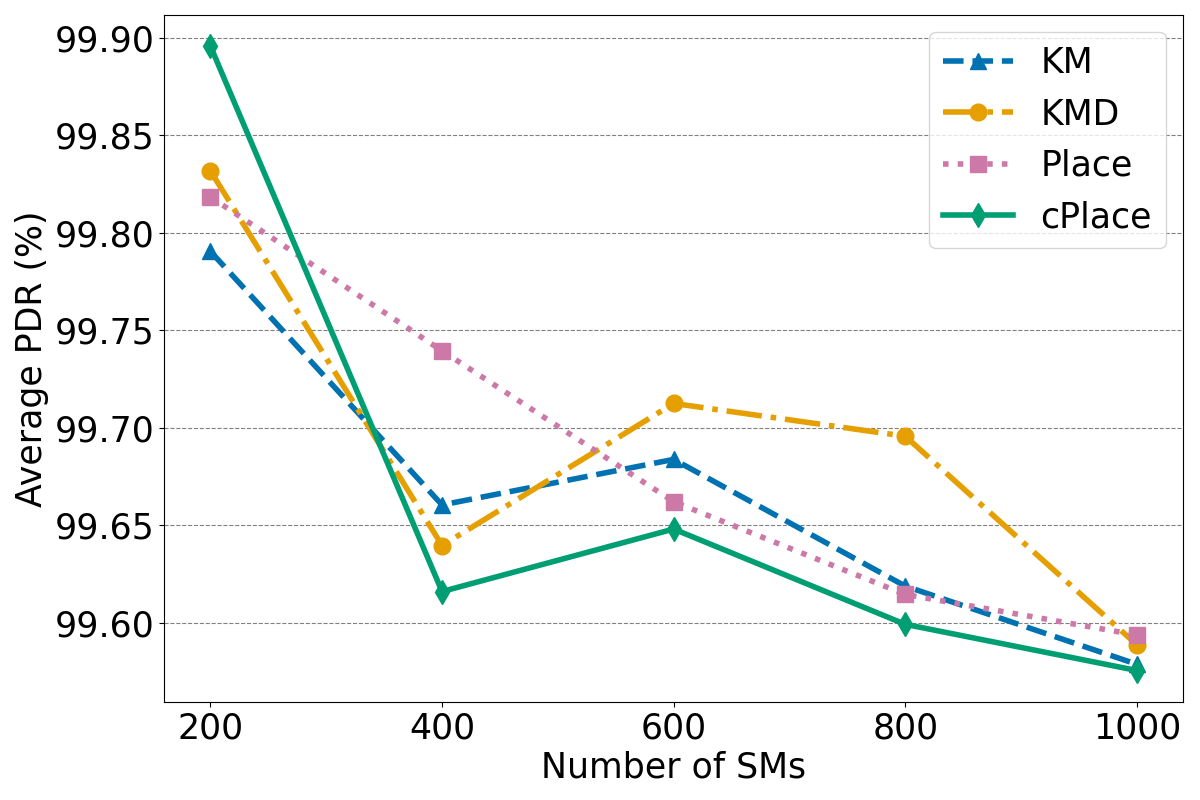
\includegraphics[width=0.98\linewidth]{imgs/pdr.png}
    \caption{LoRaWAN: Average PDR per \gls{SMs}.}
    \label{fig:pdr}
\end{figure}

%A análise das métricas delay médio e \gls{ToA} médio são apresentadas na Figura~\ref{fig:delay_toa}. O delay, descrito na Figura~\ref{fig:delay}, e o \gls{ToA}, Figura~\ref{fig:toa}, do método cPlace são menores para o cenário com 200 \gls{SMs} e depois sobem e alcançam médias similares aos dos demais métodos. 
The analysis of the average delay and the average \gls{ToA} metrics is presented in Figure~\ref{fig:delay_toa}. The delay, shown in Figure~\ref{fig:delay}, and the \gls{ToA}, shown in Figure~\ref{fig:toa}, for the cPlace method are lower in the scenario with 200 \gls{SMs}, and then increase to reach similar averages compared to the other methods.

% O delay médio de cPlace para 200 \gls{SMs} é 119.54 ms, com desvio padrão 2.90 e intervalo de confiança de 118.51 a 120.57 ms. KM tem média 121.81 ms, com desvio padrão 2.55, e intervalo de confiança entre 120.91 e 122.71 ms. Enquanto, KMD possui média 127.48 ms, desvio padrão 6.09, e intervalo de confiança de 125.32 a 129.64 ms. Por fim, Place tem média 120.90 ms, desvio padrão 3.052, e intervalo de confiança entre 119.82 e 121.99 ms.
The average delay for cPlace in the scenario with 200 \gls{SMs} is 119.54 ms, with a standard deviation of 2.90 and a confidence interval ranging from 118.51 to 120.57 ms. The KM method has an average of 121.81 ms, with a standard deviation of 2.55 and a confidence interval between 120.91 and 122.71 ms. The KMD method shows an average delay of 127.48 ms, a standard deviation of 6.09, and a confidence interval from 125.32 to 129.64 ms. Finally, the Place method has an average of 120.90 ms, a standard deviation of 3.052, and a confidence interval between 119.82 and 121.99 ms.

% O \gls{ToA} médio obtido por cPlace para 1000 \gls{SMs} é 0.34 s, com desvio padrão 0.006, e intervalo de confiança de 0.343 a 0.347 s. KM tem média 0.34 s, desvio padrão 0.007, e intervalo de confiança entre 0.342 e 0.347 s. KMD apresenta média 0.35 s, desvio padrão 0.0064, e intervalo de confiança 0.344 a 0.349 s. Por fim, Place possui média 0.345 s, com desvio padrão 0.0073, e intervalo de confiança entre 0.342 a 0.347 s.
The average \gls{ToA} obtained by cPlace for 1000 \gls{SMs} is 0.34 s, with a standard deviation of 0.006, and a confidence interval ranging from 0.343 to 0.347 s. KM has an average of 0.34 s, a standard deviation of 0.007, and a confidence interval between 0.342 and 0.347 s. KMD presents an average of 0.35 s, a standard deviation of 0.0064, and a confidence interval from 0.344 to 0.349 s. Finally, Place has an average of 0.345 s, with a standard deviation of 0.0073, and a confidence interval between 0.342 and 0.347 s.

% \begin{figure}
%     \centering
%     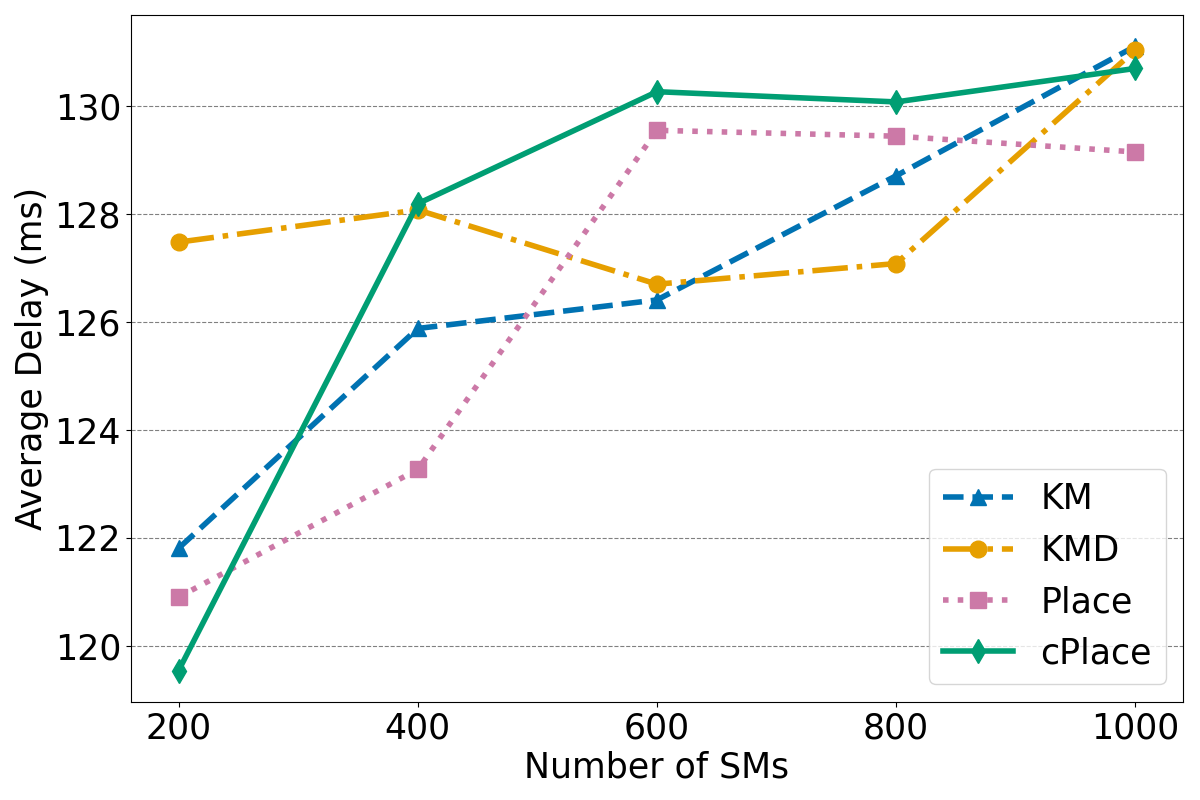
\includegraphics[width=0.99\linewidth]{imgs/delay.png}
%     \caption{Average Delay per \gls{SMs}.}
%     \label{fig:pdr}
% \end{figure}
% \begin{figure}
%     \centering
%     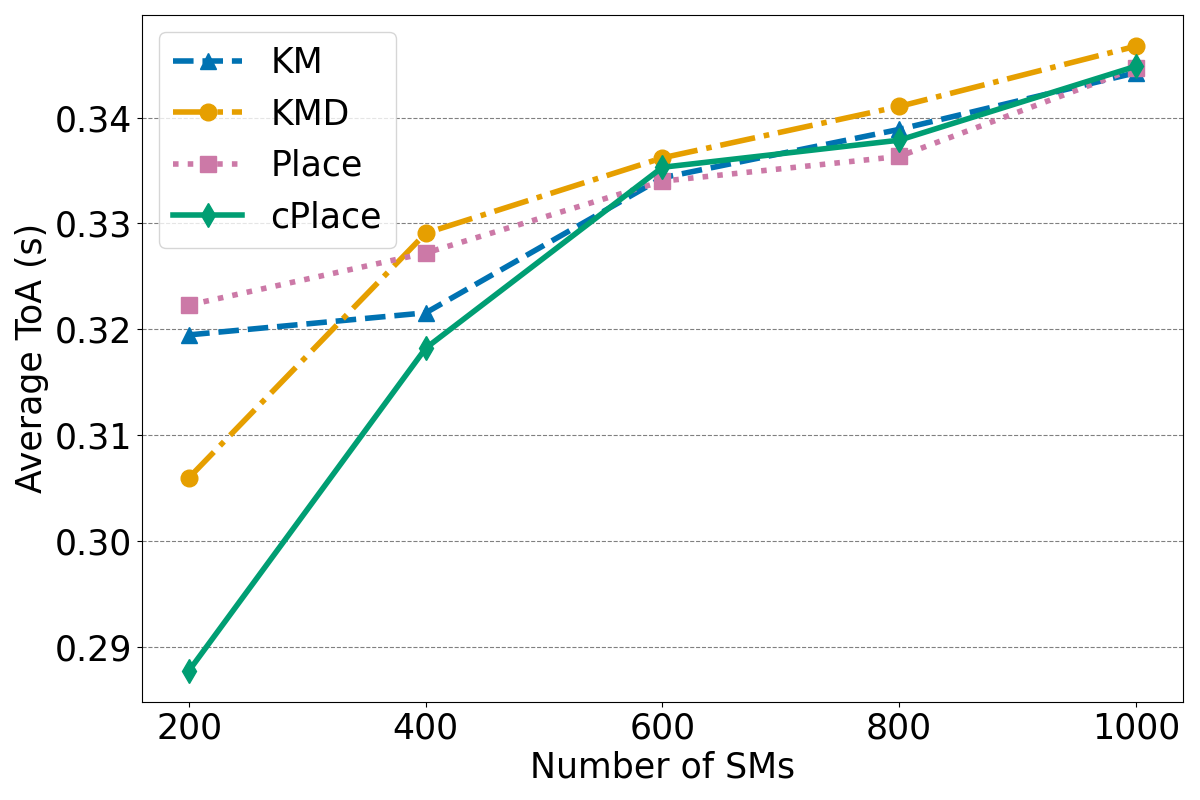
\includegraphics[width=0.99\linewidth]{imgs/toa.png}
%     \caption{Average ToA per \gls{SMs}.}
%     \label{fig:pdr}
% \end{figure}
\begin{figure}
    \centering
    \begin{subfigure}{0.48\textwidth}
        \centering
        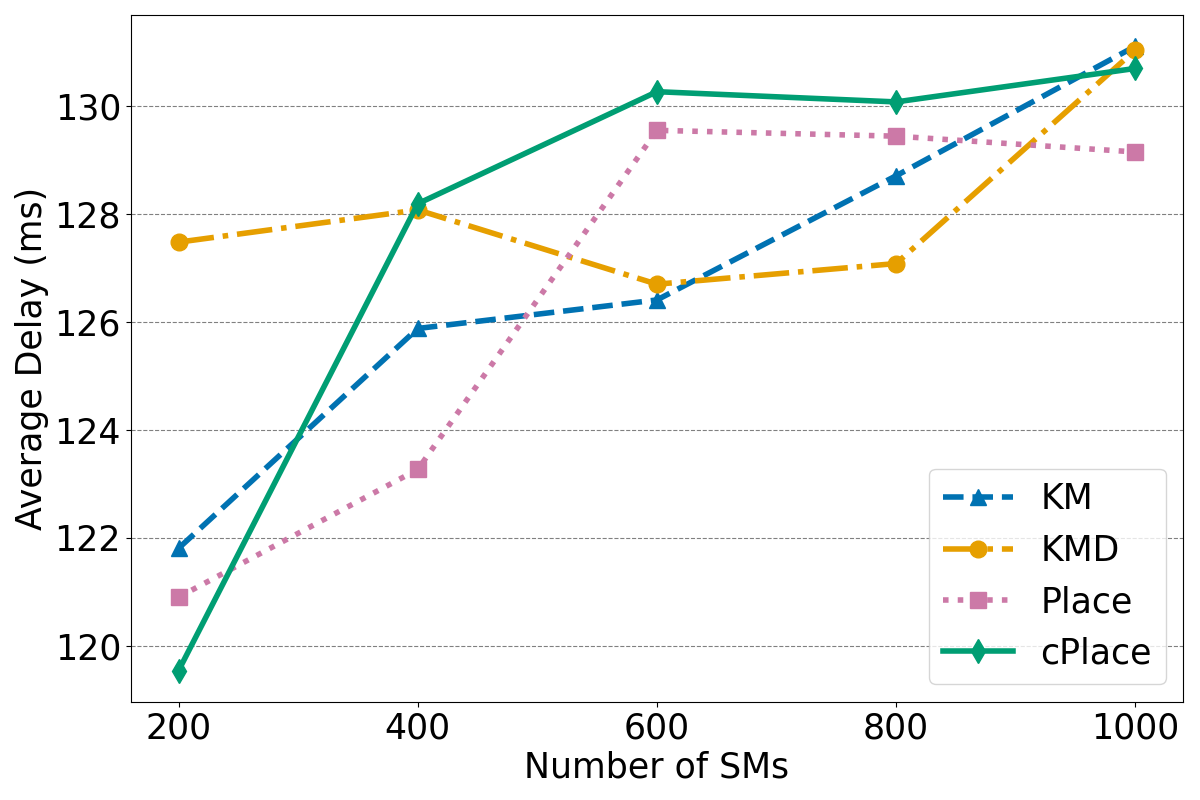
\includegraphics[width=\linewidth]{imgs/delay.png}
        \caption{Average Delay per \gls{SMs}.}
        \label{fig:delay}
    \end{subfigure}
    \hfill
    \begin{subfigure}{0.48\textwidth}
        \centering
        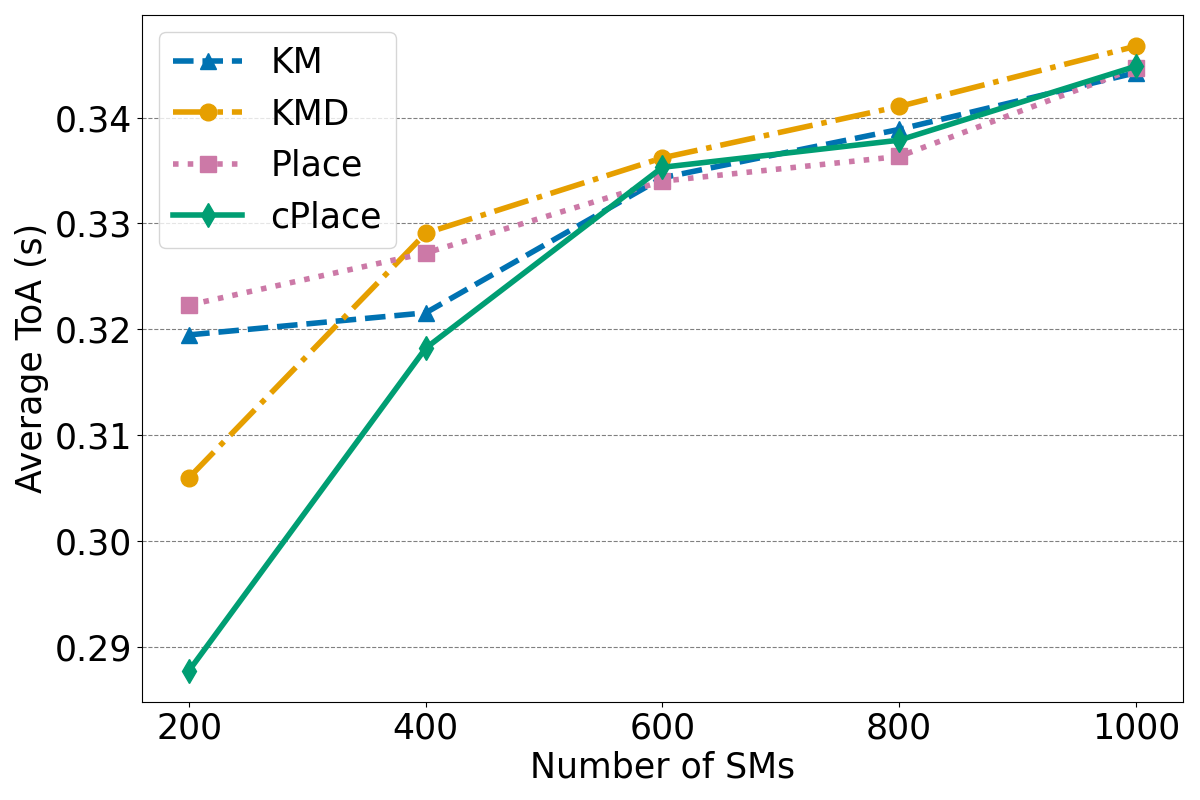
\includegraphics[width=\linewidth]{imgs/toa.png}
        \caption{Average ToA per \gls{SMs}.}
        \label{fig:toa}
    \end{subfigure}
    \caption{LoRaWAN: Analysis of the Delay and ToA.}
    \label{fig:delay_toa}
\end{figure}

%Os valores médios de consumo energético e eficiência energética são apresentadas na Figura~\ref{fig:energy_eff} e seguem o mesmo padão das figures of merit anteriores, com cPlace apresentando consumo menor para 200 \gls{SMs} e para os demais cenários a média de consumo se assemelha aos dos demais métodos. Da mesma forma, a eficiência energética média para 200 \gls{SMs} é maior e para os demais cenários as médias dos métodos se sobbrepõem.
The average energy consumption and energy efficiency values are presented in Figure~\ref{fig:energy_eff} and follow the same pattern as the previous figures of merit, with cPlace demonstrating lower consumption for 200 \gls{SMs}. In the other scenarios, the average consumption is similar to that of the other methods. Similarly, the average energy efficiency for 200 \gls{SMs} is higher, while in the other scenarios, the averages of the methods overlap.

% A Figura~\ref{fig:energy} exibe os valores de consumo energético e cPlace possi consumo médio para 200 \gls{SMs} de 11.21 J, desvio padrão 0.71, e intervalo de confiança entre 10.95 e 11.46 J. KM tem media 11.52 J, com desvio padrão de 0.25, e intervalo de confiança de 11.43 a 11.61 J. KMD apresenta média de 11.68 J, desvio padrão 0.647, e intervalo de confiança entre 11.45 e 11.90 J. Place tem média de 11.58 J, desvio padrão 0.27, e intervalo de confiança de 11.49 a 11.68 J.
Figure~\ref{fig:energy} displays the energy consumption values, where cPlace has an average consumption of 11.21 J for 200 \gls{SMs}, with a standard deviation of 0.71 and a confidence interval ranging from 10.95 to 11.46 J. KM has an average of 11.52 J, with a standard deviation of 0.25 and a confidence interval between 11.43 and 11.61 J. KMD presents an average of 11.68 J, a standard deviation of 0.647, and a confidence interval from 11.45 to 11.90 J. Place has an average of 11.58 J, a standard deviation of 0.27, and a confidence interval between 11.49 and 11.68 J.

% A Figura~\ref{fig:eff} mostra os valores médios de eficiência energética. Para o cenário com 1000 \gls{SMs}, cPlace tem média 46.89 b/s/J, desvio padrão de 0.451, e intervalo de confiança de 46.73 a 47.05 b/s/J. KM possui média de 46.94 b/s/J, desvio padrão 0.55, e intervalo de confiança de 46.74 a 47.13 b/s/J. KMD apresenta média de 46.75 b/s/J, com desvio padrão de 0.47, e intervalo de confiança de 46.58 a 46.92 b/s/J. Place possui média de 46.92 b/s/J, desvio padrão de 0.54, e intervalo de confiança de 46.73 a 47.11 b/s/J.
Figure~\ref{fig:eff} shows the average energy efficiency values. For the scenario with 1000 \gls{SMs}, cPlace has an average of 46.89 b/s/J, a standard deviation of 0.451, and a confidence interval ranging from 46.73 to 47.05 b/s/J. KM has an average of 46.94 b/s/J, a standard deviation of 0.55, and a confidence interval between 46.74 and 47.13 b/s/J. KMD presents an average of 46.75 b/s/J, with a standard deviation of 0.47, and a confidence interval from 46.58 to 46.92 b/s/J. Place has an average of 46.92 b/s/J, a standard deviation of 0.54, and a confidence interval between 46.73 and 47.11 b/s/J.

% \begin{figure}
%     \centering
%     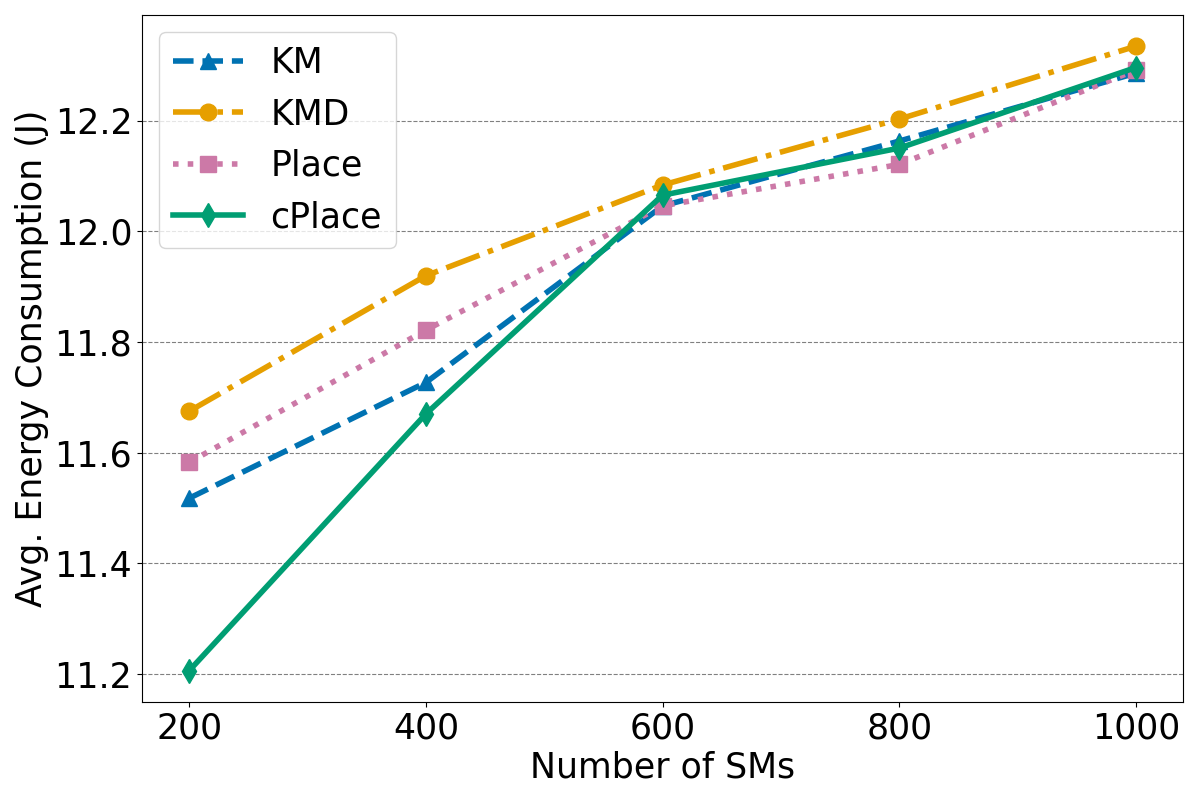
\includegraphics[width=0.99\linewidth]{imgs/energy.png}
%     \caption{Average Energy Consumption per \gls{SMs}.}
%     \label{fig:pdr}
% \end{figure}
% \begin{figure}
%     \centering
%     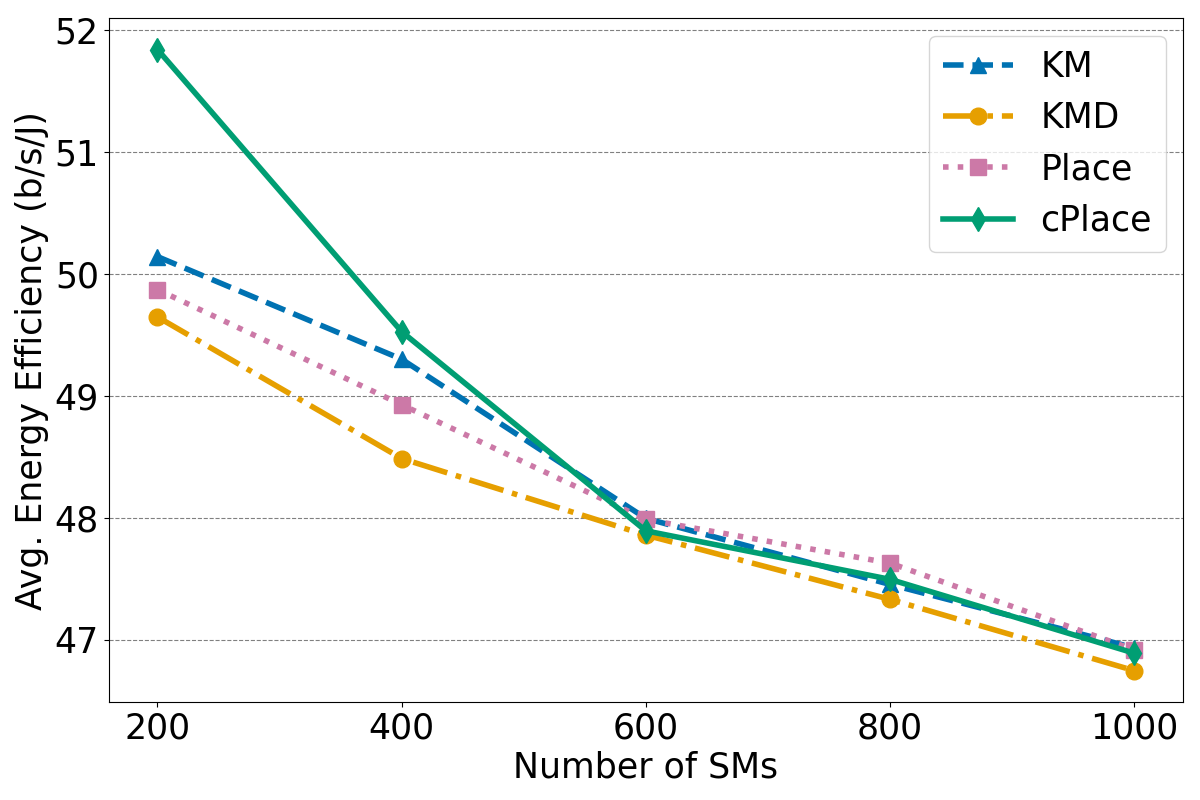
\includegraphics[width=0.99\linewidth]{imgs/eff1.png}
%     \caption{Average Energy Efficiency per \gls{SMs}.}
%     \label{fig:pdr}
% \end{figure}
\begin{figure}
    \centering
    \begin{subfigure}{0.48\textwidth}
        \centering
        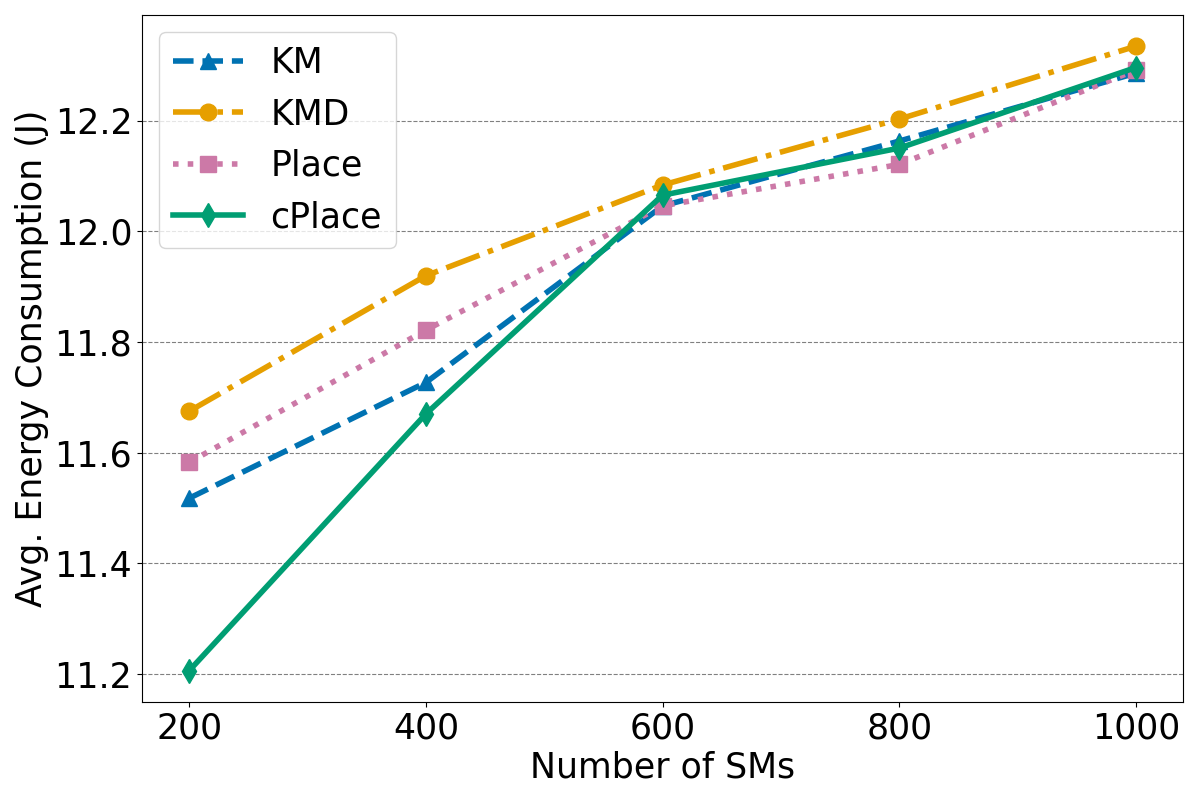
\includegraphics[width=\linewidth]{imgs/energy.png}
        \caption{Average Energy Consumption per \gls{SMs}.}
        \label{fig:energy}
    \end{subfigure}
    \hfill
    \begin{subfigure}{0.48\textwidth}
        \centering
        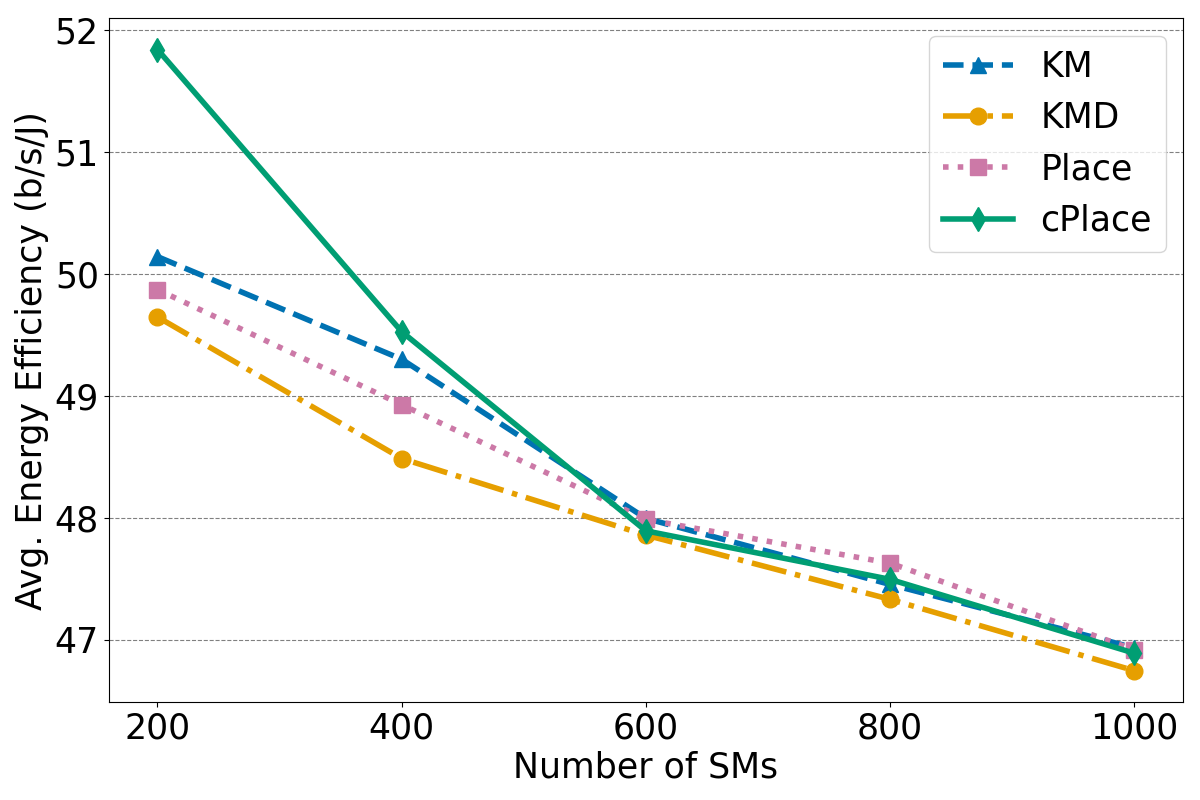
\includegraphics[width=\linewidth]{imgs/eff1.png}
        \caption{Average Energy Efficiency per \gls{SMs}.}
        \label{fig:eff}
    \end{subfigure}
    \caption{LoRaWAN: Analysis of the Energy Consumption and Energy Efficiency.}
    \label{fig:energy_eff}
\end{figure}

% A taxa de colisão média dos métodos é apresentada na Figura~\ref{fig:coll}. Com os métodos KM, Place, e cPlace tendo comportamento bem parecidos e KMD possuindo um padrão de perdas um pouco maior, mesmo apresentando uma quantidade maior de \gls{DAPs}. cPlace possui taxa média de colisão de 11.52\% para 1000 \gls{SMs}, com desvio padrão de 0.49, e intervalo de confiança variando de 11.35 a 11.69\%. KM tem média 11.49\%, com desvio padrão de 0.49, e intervalo de confiança de 11.31 a 11.66\%. KMD possui média 13.49\%, desvio padrão de 0.49, e intervalo de confiança de 13.31 a 13.66\%. Place apresenta média de 11.77\%, com desvio padrão de 0.45, e intervalo de confiança de 11.61 a 11.93\%.
The average collision rate of the methods is presented in Figure~\ref{fig:coll}. The methods KM, Place, and cPlace exhibit similar behavior, while KMD shows a slightly higher loss pattern, despite having a larger number of \gls{DAPs}. cPlace has an average collision rate of 11.52\% for 1000 \gls{SMs}, with a standard deviation of 0.49 and a confidence interval ranging from 11.35 to 11.69\%. KM has an average of 11.49\%, a standard deviation of 0.49, and a confidence interval between 11.31 and 11.66\%. KMD has an average of 13.49\%, a standard deviation of 0.49, and a confidence interval from 13.31 to 13.66\%. Place presents an average of 11.77\%, with a standard deviation of 0.45, and a confidence interval between 11.61 and 11.93\%.

\begin{figure}
    \centering
    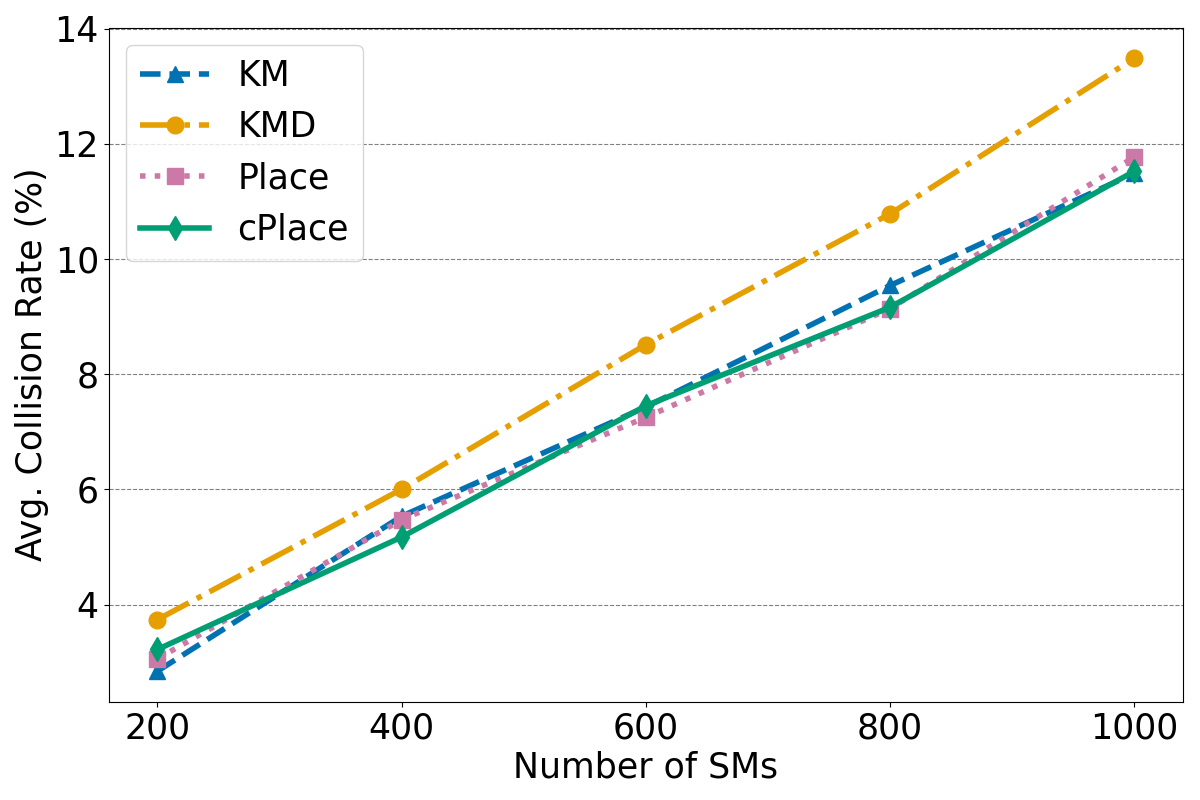
\includegraphics[width=0.99\linewidth]{imgs/coll.png}
    \caption{LoRaWAN: Analysis of the Average Collission Rate per \gls{SMs}.}
    \label{fig:coll}
\end{figure}

%A Figura~\ref{fig:rssi_snr} apresenta os valores médio de \gls{RSSI} e \gls{SNR} obtidos pelos métodos, conforme pode ser visto nas Figuras~\ref{fig:rssi} e~\ref{fig:snr}. O comportamento dessas métricas para os métods KM, Place e cPlace se assemelham bastante, com cPlace tendo indicadores médios de qualidade sinal, em alguns cenário mais baixos, pois este consegue demodular corretamente mensagens com menor intensidade e um pouco mais de ruído.
Figure~\ref{fig:rssi_snr} presents the average values of \gls{RSSI} and \gls{SNR} obtained by the methods, as shown in Figures~\ref{fig:rssi} and~\ref{fig:snr}. The behavior of these metrics for the methods KM, Place, and cPlace is quite similar, with cPlace exhibiting lower average signal quality indicators in some scenarios, as it can correctly demodulate messages with lower intensity and a more noise.

% Para o cenário com 200 \gls{SMs} cPlace tem RSSI médio de -138.43 dBm, desvio padrão de 0.12, e intervalo de confiança de -138.47 a -138.38 dBm. KM apresenta média de -138.04 dBm, desvio padrão de 0.18, e intervalo de confiança de -138.11 a -137.97 dBm. KMD possui média -137.61 dBm, desvio padrão de 0.13, e intervalo de confiança de -137.65 a -137.56 dBm. Place apresenta média de -137.44 dBm, desvio padrão de 0.15, e intervalo de confiança de -137.49 a -137.38 dBm.
For the scenario with 200 \gls{SMs}, cPlace has an average RSSI of -138.43 dBm, a standard deviation of 0.12, and a confidence interval ranging from -138.47 to -138.38 dBm. KM has an average of -138.04 dBm, a standard deviation of 0.18, and a confidence interval between -138.11 and -137.97 dBm. KMD has an average of -137.61 dBm, a standard deviation of 0.13, and a confidence interval from -137.65 to -137.56 dBm. Place presents an average of -137.44 dBm, a standard deviation of 0.15, and a confidence interval between -137.49 and -137.38 dBm.

% Para o cenário com 1000 \gls{SMs} cPlace possui SNR médio -20.21 dB, desvio padrão de 0.044, e intervalo de confiança de -20.20 a -20.23 dB. KM possui média de -20.27 dB, desvio padrão de 0.0450, e intervalo de confiança de -20.28 a -20.26 dB. KMD possui média de -18.41, desvio padrão de 0.042,e intervalo de confiança de -18.43 a -18.4 dB. Place apresenta média de -19.96 dB, desvio padrão de 0.041, e intervalo de confiança de -19.97 a -19.94 dB.
For the scenario with 1000 \gls{SMs}, cPlace has an average SNR of -20.21 dB, a standard deviation of 0.044, and a confidence interval ranging from -20.20 to -20.23 dB. KM has an average of -20.27 dB, a standard deviation of 0.0450, and a confidence interval between -20.28 and -20.26 dB. KMD has an average of -18.41 dB, a standard deviation of 0.042, and a confidence interval from -18.43 to -18.4 dB. Place presents an average of -19.96 dB, a standard deviation of 0.041, and a confidence interval between -19.97 and -19.94 dB.

% \begin{figure}
%     \centering
%     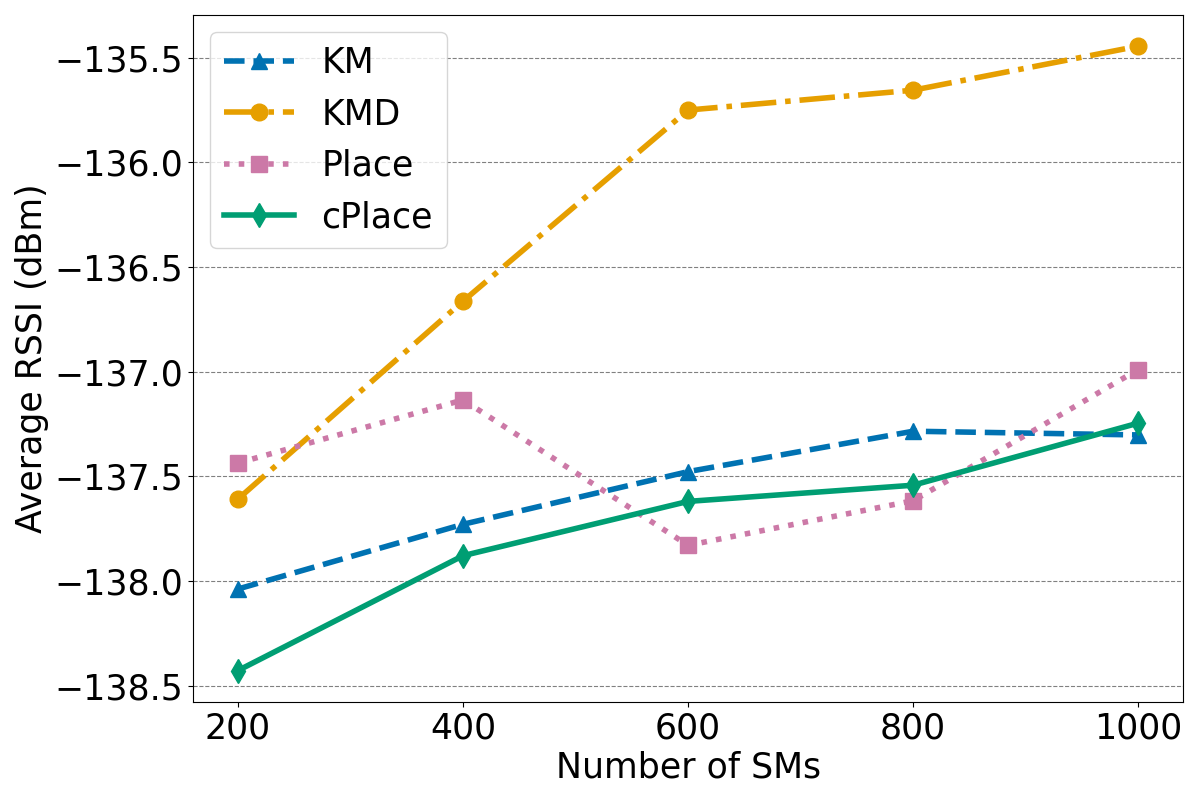
\includegraphics[width=0.99\linewidth]{imgs/rssi.png}
%     \caption{Average RSSI per \gls{SMs}.}
%     \label{fig:pdr}
% \end{figure}
% \begin{figure}
%     \centering
%     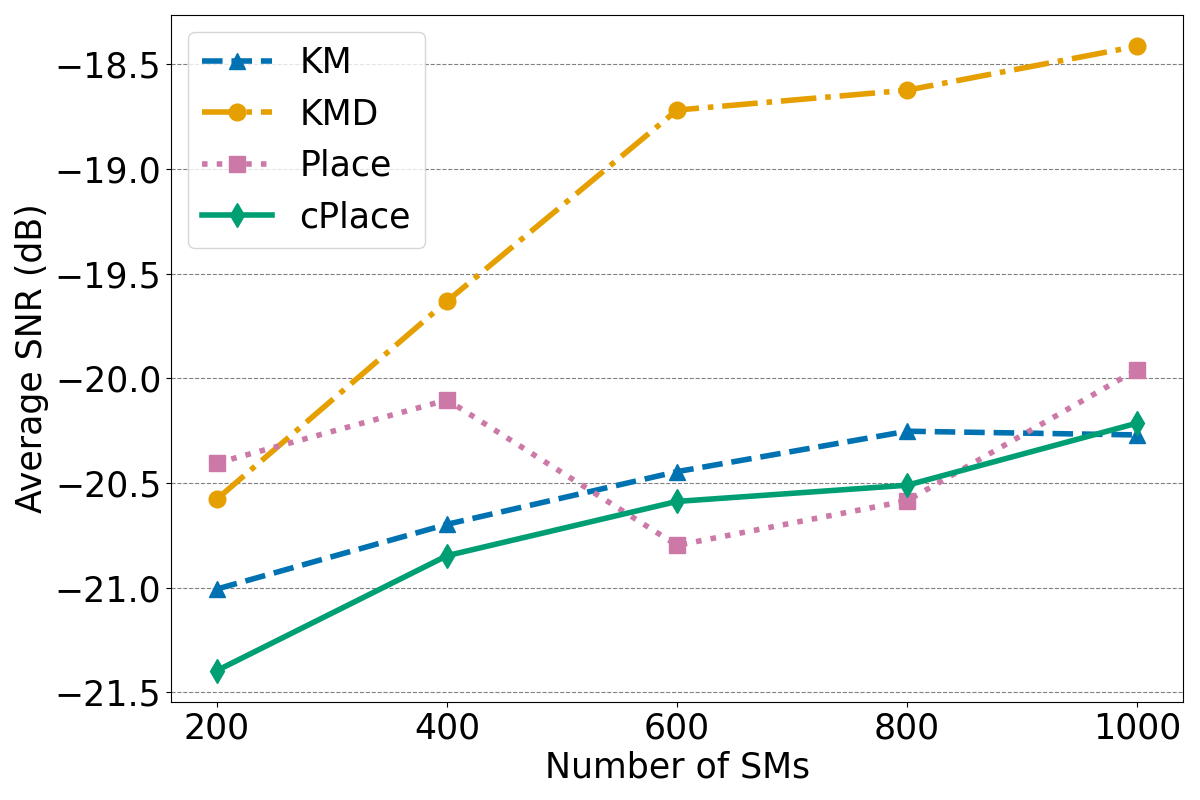
\includegraphics[width=0.99\linewidth]{imgs/snr.png}
%     \caption{Average SNR per \gls{SMs}.}
%     \label{fig:pdr}
% \end{figure}
\begin{figure}
    \centering
    \begin{subfigure}{0.48\textwidth}
        \centering
        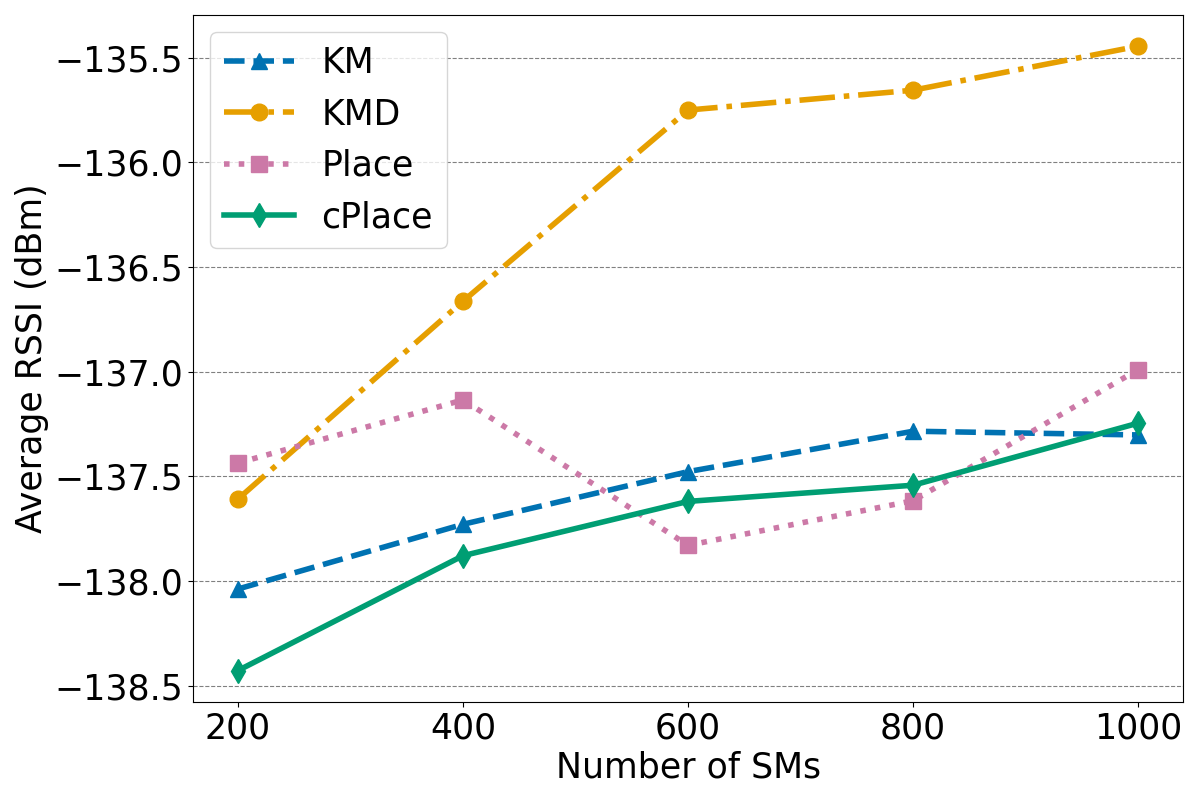
\includegraphics[width=\linewidth]{imgs/rssi.png}
        \caption{Average RSSI per \gls{SMs}.}
        \label{fig:rssi}
    \end{subfigure}
    \hfill
    \begin{subfigure}{0.48\textwidth}
        \centering
        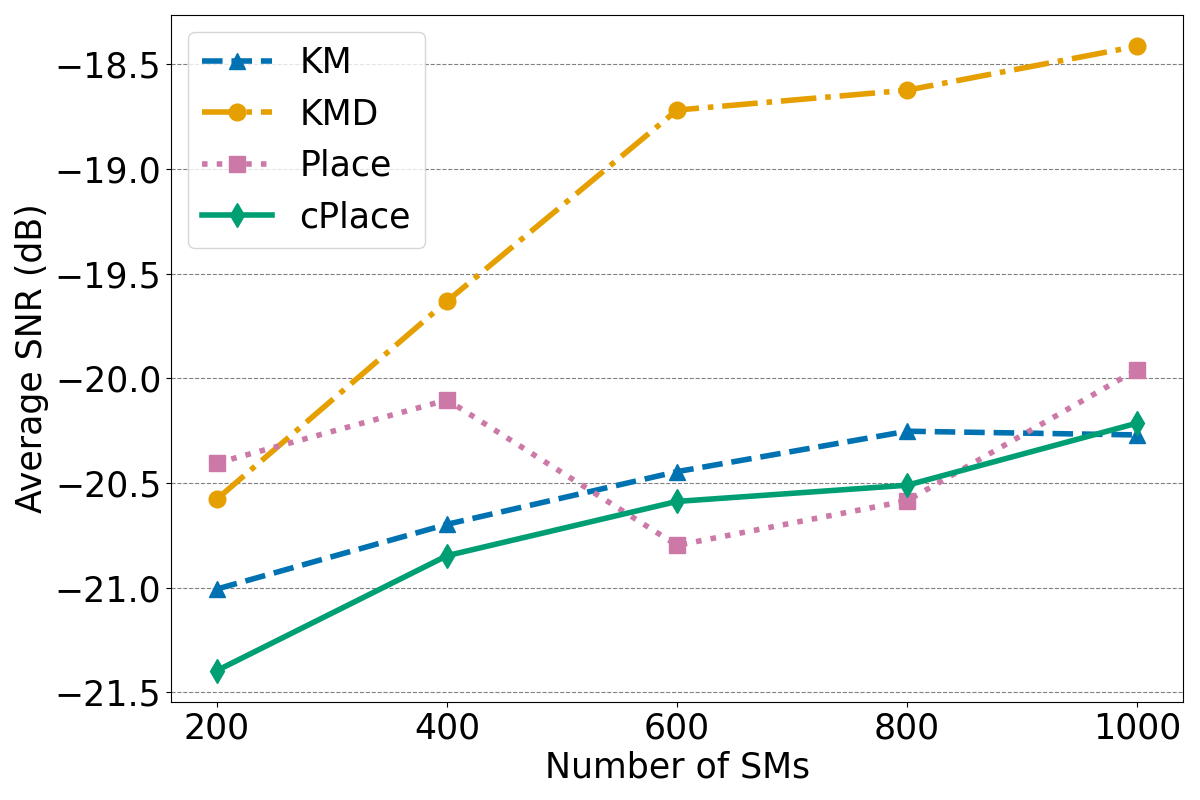
\includegraphics[width=\linewidth]{imgs/snr.png}
        \caption{Average SNR per \gls{SMs}.}
        \label{fig:snr}
    \end{subfigure}
    \caption{LoRaWAN: Analysis of the RSSI and SNR.}
    \label{fig:rssi_snr}
\end{figure}

% Com relação a análise de \gls{PLR} os métodos apresentam resultados semelhantes, com a maior parte das perdas sendo PLR-R, como pode ser visto na Figura~\ref{fig:plr}. A intuito de comparação entre os métodos, as Figuras~\ref{fig:kmd_plr} e~\ref{fig:cplace_plr} exibem as porcentagens de perdas para os métodos KMD e cPlace, respectivamente.
Regarding the analysis of \gls{PLR}, the methods show similar results, with most losses being PLR-U, as can be seen in Figure~\ref{fig:plr}. For comparison between the methods, Figures~\ref{fig:kmd_plr} and~\ref{fig:cplace_plr} display the percentages of losses for the KMD and cPlace methods for 1000 \gls{SMs}, respectively.

%KMD possui média associada ao PLR-U de 1.64\%, desvio de padrão de  0.13, e intervalo de confiança de 1.59 a 1.68\%. PLR-I tem média de 97.85\%, desvio padrão de 0.088, e intervalo de confiança de 97.82 a 97.89\%. PLR-S igual a 0. PLR-T com média 0.51\%, desvio padrão de 0.15, e intervalo de confiança de  0.45 a 0.56\%. PLR-E possui média de 0.00078\%, desvio padrão de 0.00021, e intervalo de confiança de 0.00071 a 0.00085.
KMD has an average associated with PLR-U of 1.64\%, with a standard deviation of 0.13 and a confidence interval ranging from 1.59 to 1.68\%. The average PLR-I is 97.85\%, with a standard deviation of 0.088 and a confidence interval from 97.82 to 97.89\%. The PLR-S is equal to 0. The average PLR-T is 0.51\%, with a standard deviation of 0.15 and a confidence interval ranging from 0.45 to 0.56\%. Finally, the average PLR-E is 0.00078\%, with a standard deviation of 0.00021 and a confidence interval from 0.00071 to 0.00085.

% O cPlace apresenta média para PLR-U 96.85\%, desvio padrão de 0.092, e intervalo de confiança de 96.82 a 96.89\%. PLR-I com média 2.7\%, desvio padrão de 0.14, e intervalo de confiança de 2.65 a 2.75\%. PLR-S igual a 0. PLR-T com média 0.45\%, desvio padrão de 0.12, e intervalo de confiança de 0.40 a 0.49\%. Por fim, PLR-E com média 0.00071\%, desvio padrão de 9.38e-05, e intervalo de confiança de 0.0007 a 0.00076.
cPlace has an average PLR-U of 96.85\%, with a standard deviation of 0.092 and a confidence interval ranging from 96.82 to 96.89\%. The average PLR-I is 2.7\%, with a standard deviation of 0.14 and a confidence interval from 2.65 to 2.75\%. The PLR-S is equal to 0. The average PLR-T is 0.45\%, with a standard deviation of 0.12 and a confidence interval ranging from 0.40 to 0.49\%. Finally, the average PLR-E is 0.00071\%, with a standard deviation of 9.38e-05 and a confidence interval from 0.0007 to 0.00076.

\begin{figure}
    \centering
    \begin{subfigure}{0.48\textwidth}
        \centering
        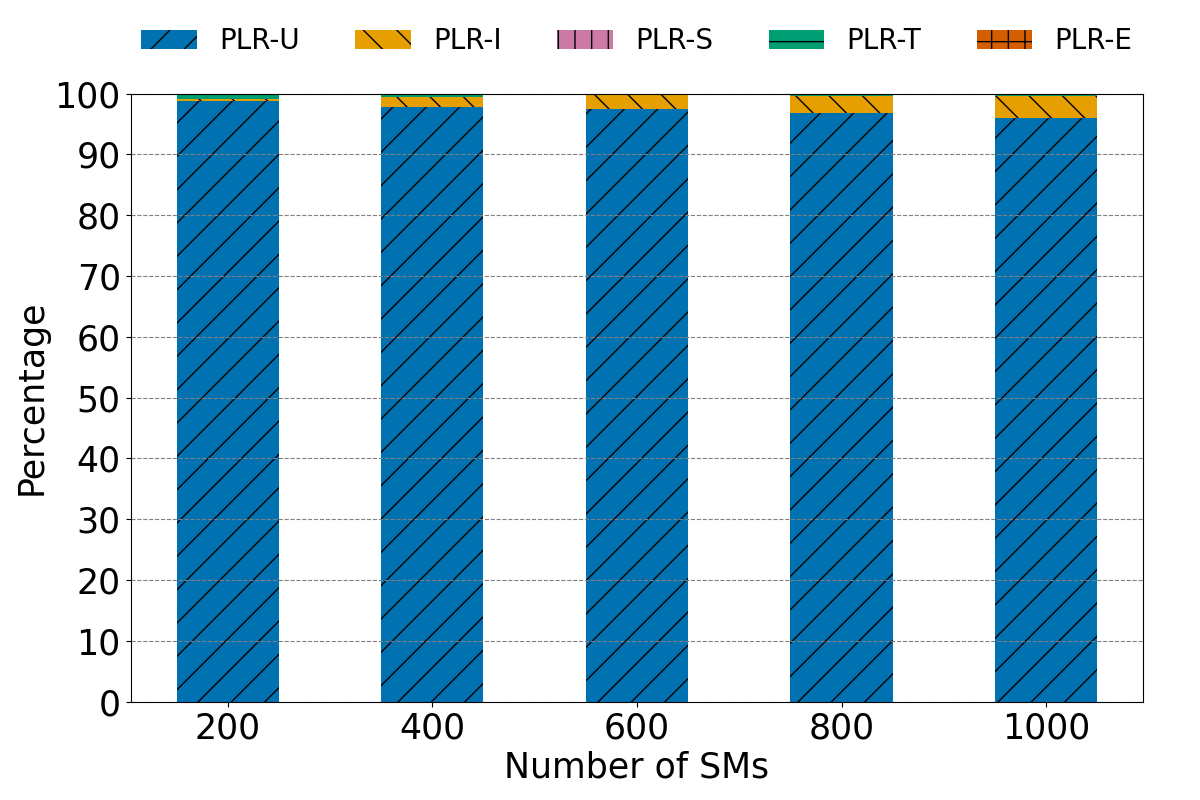
\includegraphics[width=\linewidth]{imgs/kmd_plr.png}
        \caption{PLR of the KMD Method for 1000 \gls{SMs}.}
        \label{fig:kmd_plr}
    \end{subfigure}
    \hfill
    \begin{subfigure}{0.48\textwidth}
        \centering
        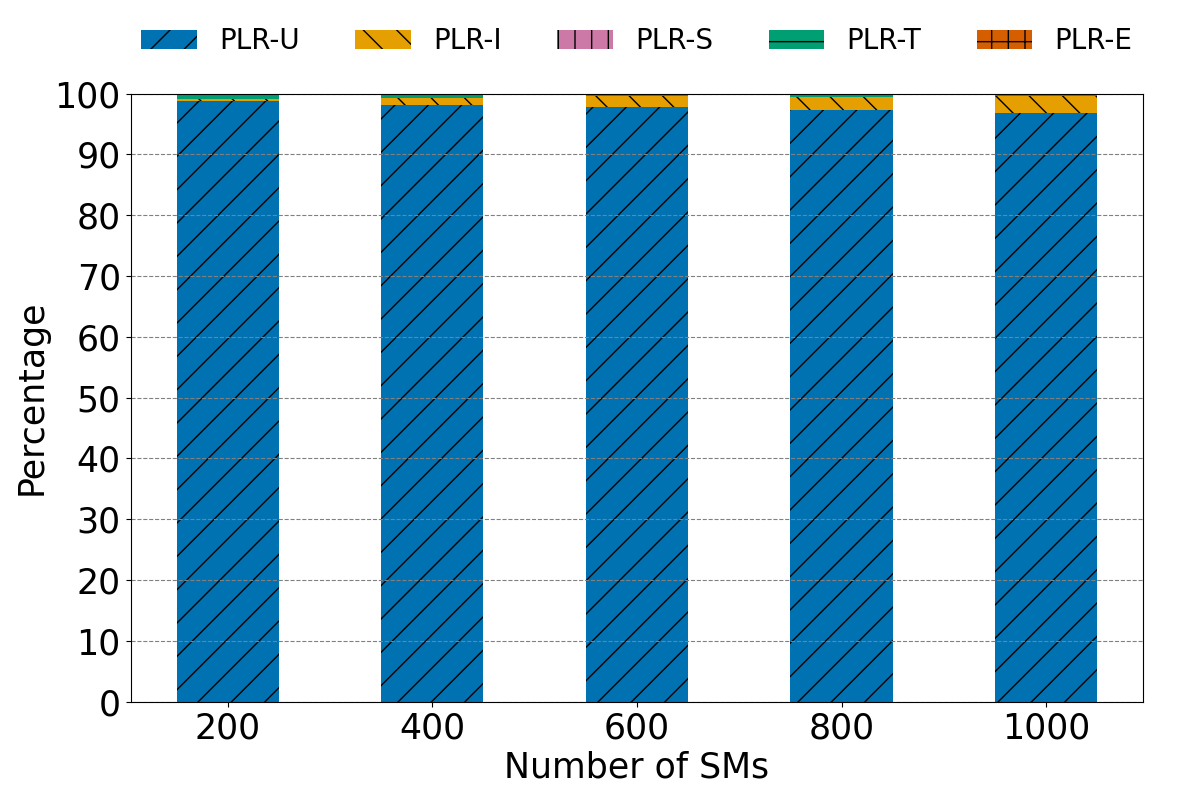
\includegraphics[width=\linewidth]{imgs/cplace_plr.png}
        \caption{PLR of the cPlace Method for 1000 \gls{SMs}.}
        \label{fig:cplace_plr}
    \end{subfigure}
    \caption{LoRaWAN: Analysis of the Average PLR.}
    \label{fig:plr}
\end{figure}

%Um exemplo da distribuição final dos SFs gerados pelos métodos é apresentado na Tabela~\ref{tab:sf_dist}, que exibe as porcentagens de SFs alocados para os 1000 \gls{SMs} para o método cPlace e os três métodos alternativos. Os valores demonstram que mais de 99\% dos \gls{SMs} para todos os métodos utilizam SF7, e um pequena porcentagem aplicam SF8, com o método KMD destoando um pouco dos demais e possuindo \gls{SMs} com SF9, o que indica que este método apresenta um \gls{ToA} ligeiramente maior. Os demais SFs são omitidos, pois não são utilizados.
An example of the final \gls{SF} distribution generated by the methods is presented in Table~\ref{tab:sf_dist}, which shows the percentages of SFs allocated to the 1000 \gls{SMs} for the cPlace method and the three alternative methods. The results demonstrate that more than 99\% of the \gls{SMs} for all methods use SF7, and a small percentage apply SF8, with the KMD method slightly diverging from the others by having \gls{SMs} with SF9, indicating that this method results in a slightly higher \gls{ToA}. The remaining SFs are omitted, as they are not used.

\begin{table}[ht]
    \centering
    \caption{LoRaWAN: Distribution of SFs for 1000 \gls{SMs} (\%).}
    \begin{tabular}{ccccc}
        \hline \hline
        \gls{SF} &  KM & KMD & Place & cPlace \\ \hline
           7      &  99.994 & 99.797 & 99.979 & 99.958 \\
           8      &  0.006 &  0.188 & 0.021 & 0.042 \\
           9      &  0  &  0.15 & 0 & 0 \\ \hline \hline
          %10      &  0 &  0 & 0 & 0 \\ 
          %11      &  0 &  0 &  0 & 0 \\ 
          %12      &  0  &  0 &  0 & 0 \\ \hline \hline
    \end{tabular}
    \label{tab:sf_dist}
\end{table}

%Os valores de CAPEX para cada um métodos, com relação aos cenários com as diferentes quantidades de \gls{SMs}, são apresentados na Tabela~\ref{tab:capex}. O método cPlace possuem custos menores em todos os cenários, mesmo que compartilhando o mesmo valor em k\EUR{} com outros métodos. No cenário com 600 \gls{SMs} o custo é o menor dentre todos e é igual a 120.7~k\EUR{} e no cenário com 1000 \gls{SMs} o custo de \gls{CAPEX} obtido, assim como o do método KM é 142.0, o que indica que a estratégia de posicionamento dos \gls{DAPs} considerando o \gls{PDR} é uma estratégia que corrobora para melhoria da performance da comunicação.
The \gls{CAPEX} values for each method, in relation to the scenarios with different numbers of \gls{SMs}, are presented in Table~\ref{tab:capex}. The cPlace method has lower costs in all scenarios, even when sharing the same value in k\EUR{} with other methods. In the scenario with 600 \gls{SMs}, the cost is the lowest among all, at 120.7~k\EUR{}, and in the scenario with 1000 \gls{SMs}, the \gls{CAPEX} cost obtained, as well as that of the KM method, is 142.0~k\EUR{}. This indicates that the \gls{DAPs} positioning strategy based on the \gls{PDR} metric contributes to improving communication performance.

\begin{table}[ht]
    \centering
    \caption{\gls{CAPEX} per Number of \gls{SMs} (in k\EUR{}).}
    \begin{tabular}{ccccc}
        \hline \hline
        \gls{SMs} &  KM & KMD & Place & cPlace \\ \hline
        200      &  99.40 &  92.3 & 113.6 & 92.3 \\
        400      &  99.40 &  113.6 & 120.7 & 92.3 \\
        600      &  134.9 &  191.7 & 120.7 & 120.7 \\ 
        800      &  134.9 &  191.7 & 127.8 & 127.8 \\ 
        1000     &  142.0 &  191.7 &  149.1 & 142.0 \\ \hline \hline
    \end{tabular}
    \label{tab:capex}
\end{table}

Finally, the \gls{OPEX} values for each method in relation to the different test scenarios are presented in Table~\ref{tab:opex} and follow the same pattern described in the \gls{CAPEX} analysis. Thus, the \gls{OPEX} values for the cPlace method considering 200 and 400 \gls{SMs} are 38.84~\text{k\EUR{}$/$year}, and the cost for the scenario with 1000 \gls{SMs} is 59.75~\text{k\EUR{}$/$year}.

\begin{table}[ht]
    \centering
    \caption{\gls{OPEX} per Number of \gls{SMs} (in \text{k\EUR{}$/$year}).}
    \begin{tabular}{ccccc}
        \hline \hline
        \gls{SMs} &  KM & KMD & Place & cPlace \\ \hline
        200      &  41.83 &  38.84 & 47.8 & 38.84 \\
        400      &  41.83 &  47.8 & 50.79 & 38.84 \\
        600      &  56.76 &  80.66 & 50.78 & 50.79 \\ 
        800      &  56.76 &  80.66 & 53.78 & 53.79 \\ 
        1000     &  59.75 &  80.66 & 62.74 & 59.75 \\ \hline \hline
    \end{tabular}
    \label{tab:opex}
\end{table}

\section{Conclusion and Future Works} \label{sec:conclusion}

This paper proposes a method, named cPlace, to determine the quantity and positions \gls{DAPs} de um \gls{AMI} system, with the aim of ensuring the proper operation of \gls{AMI} applications. The proposed method and related solutions are tested through simulations, and after executing them, the values of the evaluation metrics are obtained.

%The cPlace method defines an infrastructure with até 37.04\% less \gls{DAPs} compared to the KMD method KMD para o cenário com 600 \gls{SMs}. Additionally, cPlace achieves similar values to the other methods for the metrics of avaliação da performance da rede LoRaWAN, despite utilizing less \gls{DAPs}.
The cPlace method defines an infrastructure with up to 37.04\% fewer \gls{DAPs} compared to the KMD method for the scenario with 600 \gls{SMs}. Additionally, cPlace achieves similar values to the other methods for the performance evaluation metrics of the LoRaWAN network, despite utilizing fewer \gls{DAPs}.

%Furthermore, the results highlight the applicability of network operation metrics combined with the coordinates of \gls{SMs} to improve the positioning of \gls{DAPs}. Finally, as future work, the prototyping of the proposed method in a real environment should be carried out, bem como investigar mecanismos para distribuição dos SFs a fim de reduzir a quantidade de colisões.
Furthermore, the results highlight the applicability of network operation metrics combined with the coordinates of \gls{SMs} to improve the positioning of \gls{DAPs}. Finally, as future work, the prototyping of the proposed method in a real environment should be carried out, as well as investigating mechanisms for the distribution of SFs to reduce the number of collisions.

% \appendix
% \section{My Appendix}
% Appendix sections are coded under \verb+\appendix+.

% \verb+\printcredits+ command is used after appendix sections to list 
% author credit taxonomy contribution roles tagged using \verb+\credit+ 
% in frontmatter.

\printcredits

\section*{Declaration of competing interest}

The authors declare that they have no known competing financial interests or personal relationships that could have appeared to influence the work reported in this paper.

\section*{Data availability}

Data will be made available on request.

%% Loading bibliography style file
%\bibliographystyle{model1-num-names}
\bibliographystyle{cas-model2-names}

% Loading bibliography database
\bibliography{cas-refs}


%\vskip3pt

% \bio{}
% Author biography without author photo.
% Author biography. Author biography. Author biography.
% Author biography. Author biography. Author biography.
% Author biography. Author biography. Author biography.
% Author biography. Author biography. Author biography.
% Author biography. Author biography. Author biography.
% Author biography. Author biography. Author biography.
% Author biography. Author biography. Author biography.
% Author biography. Author biography. Author biography.
% Author biography. Author biography. Author biography.
% \endbio

% \bio{figs/pic1}
% Author biography with author photo.
% Author biography. Author biography. Author biography.
% Author biography. Author biography. Author biography.
% Author biography. Author biography. Author biography.
% Author biography. Author biography. Author biography.
% Author biography. Author biography. Author biography.
% Author biography. Author biography. Author biography.
% Author biography. Author biography. Author biography.
% Author biography. Author biography. Author biography.
% Author biography. Author biography. Author biography.
% \endbio

% \bio{figs/pic1}
% Author biography with author photo.
% Author biography. Author biography. Author biography.
% Author biography. Author biography. Author biography.
% Author biography. Author biography. Author biography.
% Author biography. Author biography. Author biography.
% \endbio

\end{document}

+